%% LyX 2.3.6.1 created this file.  For more info, see http://www.lyx.org/.
%% Do not edit unless you really know what you are doing.
\documentclass[english]{article}
\usepackage[T1]{fontenc}
\usepackage[latin9]{inputenc}
\usepackage{geometry}
\geometry{verbose,tmargin=3.5cm,bmargin=2.5cm,lmargin=2.5cm,rmargin=2.5cm,headsep=0.5cm,footskip=1cm}
\usepackage{float}
\usepackage{url}
\usepackage{amsmath}
\usepackage{graphicx}
\usepackage{setspace}

\makeatletter
\@ifundefined{date}{}{\date{}}
\makeatother

\usepackage{babel}
\usepackage{listings}
\renewcommand{\lstlistingname}{Listing}

\begin{document}
\title{Side-channel evaluation of Shakti's AES accelerators}
\author{Surya Prasad S (Guided by Chester Rebeiro)}
\maketitle
\begin{center}
\url{https://github.com/GnosGnas/Side-Channel-Analysis}
\par\end{center}

\begin{singlespace}
\index{Table of Contents}{\footnotesize{}\tableofcontents{}}{\footnotesize\par}
\end{singlespace}

\pagebreak{}

\section{Introduction}

Power Analysis attacks have proven to be fatal to otherwise tamper-proof
hardware. Non-invasive attacks like SPA and DPA are particularly dangerous
as they can be easily reproduced and scaled. So, enter Test Vector
Leakage Assessment Methodology (TVLA), a popular side-channel testing
methodology as it can detect power leakages at any time of the operation
irrespective of whether an attack can be successfully performed or
not with that leakage. Test Vector Leakage Assessment (TVLA) aims
to provide detection of information leakage using statistical analysis.
We have done the TVLA test on Shakti's AES accelerators which can
be integrated with the Shakti C-Class processor. The power consumption
of our AES accelerators have been analysed extensively and optimisations
are made to reduce power leakage. 

\section{Overview}

\subsection{AES Algorithm }

Advanced Encryption Standard, or AES, is a popular symmetric algorithm
for encryption. Symmetric algorithms are named because they use the
same cryptographic key for encryption and decryption. This comes with
both advantages and disadvantages. From an implementation point of
view, symmetric algorithms process much quicker than asymmetric algorithms,
and a typical hardware accelerator takes only 12 cycles to complete
one process.

The algorithm takes in a 128-bit input and generates a 128-bit output.
AES is capable of using keys of length 128, 192 or 256 bits. The algorithm
encrypts or decrypts by repeatedly applying a set of operations to
the input data. The number of rounds of a process is fixed for each
length of key:
\begin{itemize}
\item 10 rounds for AES-128
\item 12 rounds for AES-192
\item 14 rounds for AES-256
\end{itemize}
\pagebreak Figure 1 shows the structure of AES algorithm and specifies
the operations in each round.

\begin{figure}[H]
\noindent \begin{centering}
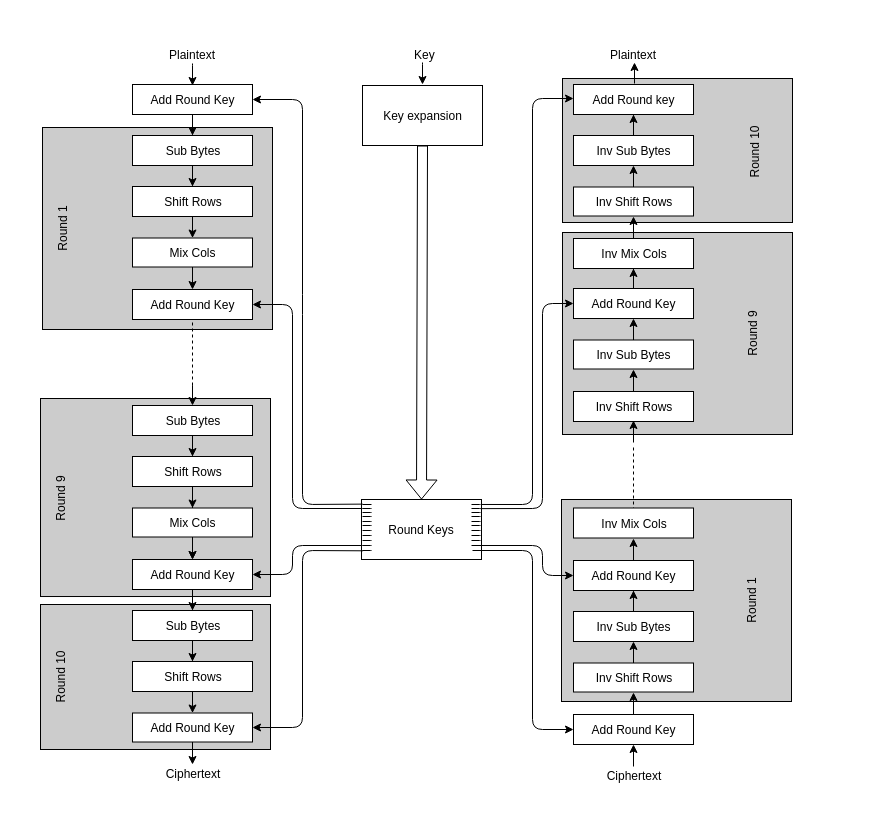
\includegraphics[scale=0.3]{report_pictures/AES_flow}
\par\end{centering}
\caption{Algorithmic structure of 128-bit AES}

\end{figure}

\emph{SubBytes} and \emph{InvSubBytes} are two critical functions
in encryption and decryption. They use the transformation function
S-box, which consumes a great deal of power in the AES algorithm's
hardware and software implementations.

\subsubsection{SubBytes}

\emph{SubBytes} transformation \cite{key-1} is a non-linear byte
substitution that maps one byte to another in $GF(2^{8})$. The mapping
of each byte is done using an S-box which is defined over the irreducible
polynomial, $R(x)=x^{8}+x^{4}+x^{3}+x+1$. The output of the S-box
is defined as follows:
\noindent \begin{center}
$SBox(a)=\begin{cases}
\begin{array}{c}
Ma^{-1}+N\\
N
\end{array} & \begin{array}{c}
if\:a\neq0\\
if\:a=0
\end{array}\end{cases}$
\par\end{center}

where M is an $8x8$ matrix, $N\in GF(2^{8})$ and $a^{-1}$ is the
multiplicative inverse in $GF(2^{8})$. 

There exists an isomorphism between $GF(2^{8})$ and composite field
of the same cardinality, which we have taken advantage of in our implementation. 

\begin{table}[H]
\caption{AES S-box Table}

\centering{}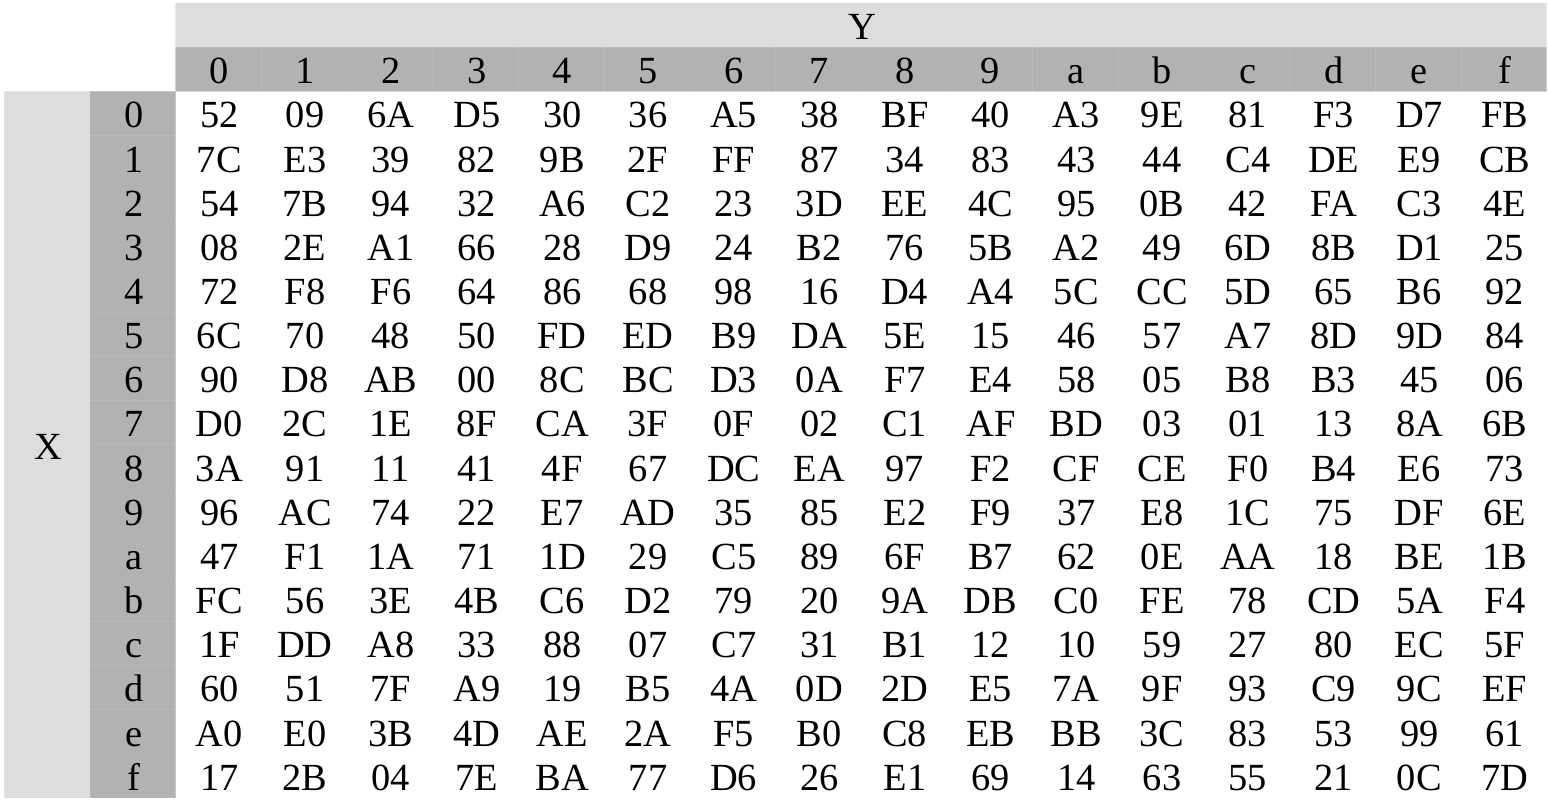
\includegraphics[scale=0.25]{report_pictures/sboxnew}
\end{table}


\subsubsection{InvSubBytes }

\emph{InvSubBytes} \cite{key-1} is the inverse of the byte substitution
transformation and maps one byte to another using the inverse S-box.
Inverse S-box is defined as follows:
\noindent \begin{center}
$InvSBox(b)=\begin{cases}
\begin{array}{c}
M^{-1}(b+N)^{-1}\\
0
\end{array} & \begin{array}{c}
if\:b\neq N\\
if\:b=N
\end{array}\end{cases}$
\par\end{center}

where similar definitions are followed.

Here too we can utilize the isomorphism with composite field arithmetic.

\begin{table}[H]
\caption{AES Inverse S-box Table}

\noindent \centering{}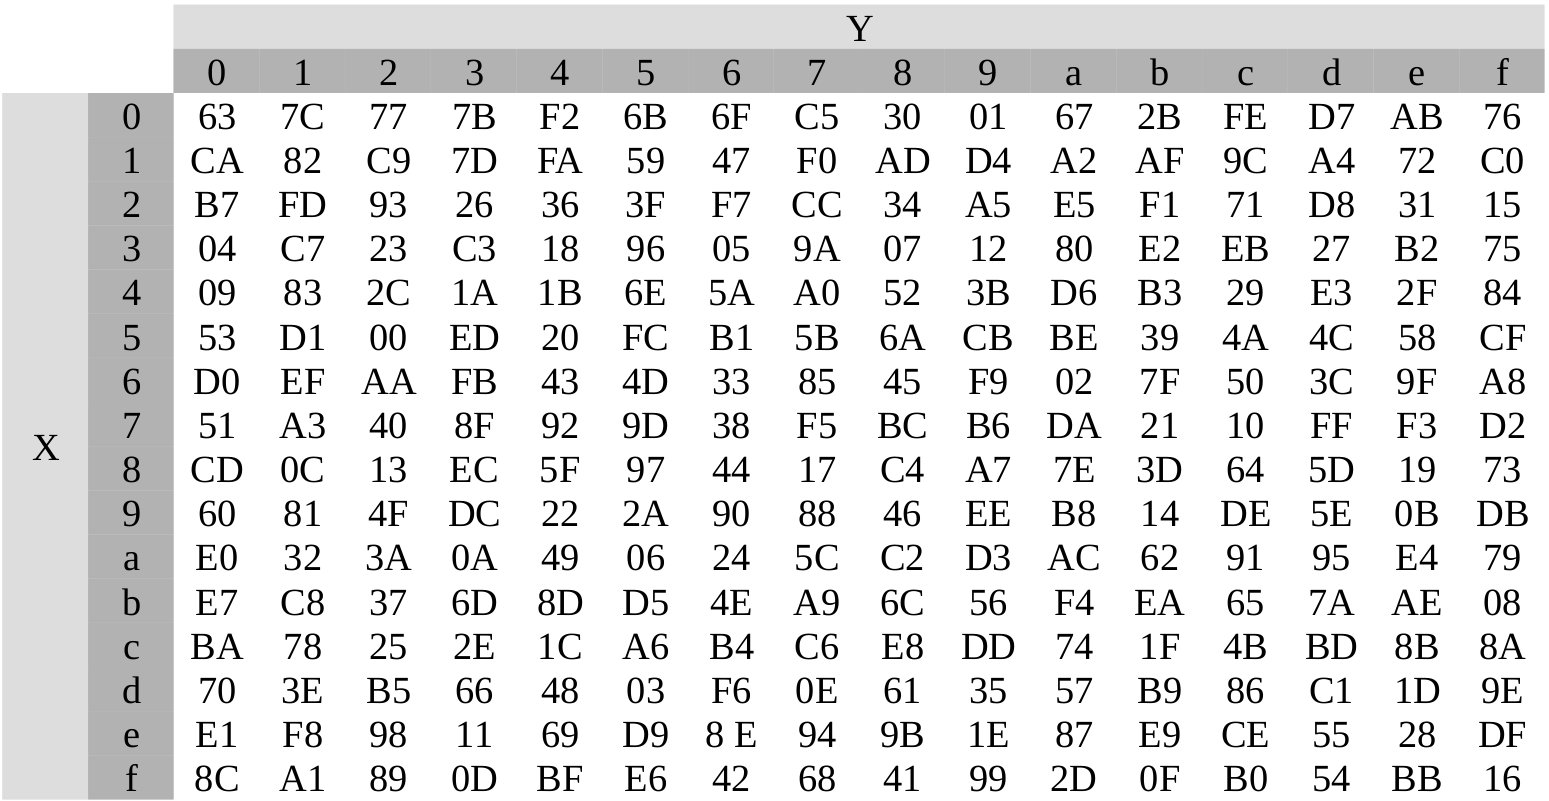
\includegraphics[scale=0.25]{report_pictures/invsboxnew}
\end{table}

\pagebreak{}

\subsection{Side-channel attacks}

A side-channel attack attempts to gather information or influence
the program execution of a system by measuring or exploiting the physical
nature of the system or its hardware. There are various known attacks,
and the most common attacks are:
\begin{itemize}
\item Timing attack
\item Electromagnetic (EM) attack
\item Simple Power Analysis (SPA)
\item Differential Power Analysis (DPA)
\item Template attack
\end{itemize}
In this section, we shall briefly cover SPA and DPA power attacks.

\subsubsection{Simple Power Analysis (SPA)}

Simple Power Analysis (SPA) is a side-channel attack that involves
visual examination of graphs of the current used by the device over
time. Variations in the graph allow the attacker to determine the
secret key. Very few power traces are required, and usually, a single
plaintext is passed multiple times, and the mean power trace is analysed.
Consider a SPA attack on the RSA algorithm, a popular asymmetric algorithm.
Multiplication is carried out when the $i_{th}$ bit of the private
key is one else a square operation is performed. So if the power trace
of multiplication and square is differentiable, the attacker will
be able to reveal the $i_{th}$ bit and eventually the attacker will
be able to reveal the whole key.

\subsubsection{Differential Power Analysis (DPA)}

Differential Power Analysis (DPA) attacks are among the most popular
power analysis attacks. This is because the implementation details
of the attacked device are not required in great detail. Furthermore,
DPA can reveal the secret key even in the presence of a large amount
of noise. In contrast to SPA attacks, DPA attacks would require a
large number of traces. In a DPA attack \cite{key-7}, the attacker
analyses how fixed time instances depend on the processed data. There
are five steps involved:
\begin{enumerate}
\item Choose an intermediate result as a function $f(d,k)$, where $d$
is the data value (either plaintext or ciphertext) and $k$ is a byte
of the key.
\item Measure the power consumption while running encryption or decryption
on the device, and the data set can be represented as a 2-D array
S{[}$N_{D}${]}{[}$N_{T}${]}, where $N_{D}$ is the total number
of data values and $N_{T}$ is the total length of the trace.
\item Construct a differential average trace T from the data set S.
\item The intermediate results are then mapped to the hypothetical power
consumption values, H.
\item Finally, the hypothetical values H are compared with the measured
power consumption values using statistical tools like correlation
and R matrix is generated. The indices of the highest values of the
matrix R are used to reveal the positions at which the chosen intermediate
result has been processed and the key used by the device. If all the
values are approximately equal, then more traces are needed.
\end{enumerate}

\subsubsection{NIST's Side-Channel Conformance Test}

No testing program can guarantee resistance against all attacks, but
a practical approach should be able to validate the security of the
hardware implementation. The following are the requirements for an
effective validation test \cite{key-6}:
\begin{itemize}
\item Effectiveness of tests: Reproducible results and reasonable conditions
of testing
\item Ease and cost-effectiveness of testing: Should not take an excessive
amount of time or require exceptional test operator skills
\end{itemize}
Test Vector Leakage Assessment (TVLA) is a popular conformance style
testing methodology recommended by NIST due to its robustness and
ease of implementing and integrating it for various crypto-implementations
with existing methodologies.

\subsubsection{Test Vector Leakage Assessment (TVLA)}

TVLA uses Welch's t-test, a PASS/FAIL test that checks if t-value
crosses a predefined threshold (proposed as $\pm4.5$). If the t-value
crosses the threshold, there is a possibility of data leakage at that
particular instant of time. It is to be noted that this is not sufficient
to objectively tell that the device leaks data, which can be confirmed
only by performing side-channel attacks. This is particularly true
with processors as they may have multiple power leakage sources unrelated
to the actual crypto-code that might be running. The testing strategy
can be summarised as follows.

\begin{figure}[H]
\noindent \begin{centering}
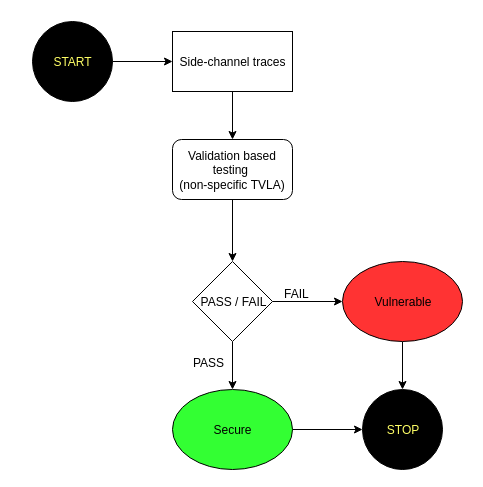
\includegraphics[scale=0.5]{report_pictures/TVLA_flow}
\par\end{centering}
\caption{Testing methodology for non-specific TVLA}

\end{figure}

The ideal TVLA score (maximum t-value) should be 0, and this is the
case when the mean of two sets of power traces corresponding to a
fixed input and a random input are equal, which implies that the power
consumed by different inputs is the same on an average at any point
of time. The t-values are given using the following equation as shown
below.
\noindent \begin{center}
$t=\frac{\mu_{A}-\mu_{B}}{\sqrt{\frac{\sigma_{A}^{2}}{n_{A}}+\frac{\sigma_{B}^{2}}{n_{B}}}}$,
where $\mu$ and $\sigma$ are mean and standard deviations of corresponding
sets A and B.
\par\end{center}

Ideally, the variance for the fixed data should be 0, but there will
be some variance due to physical randomness. High variance for fixed
data will lead to a lower TVLA score which is expected as it implies
higher unpredictability of identifying the immediate values. We also
note the effect of the number of traces and theoritically the t-value
increase proportional to $\sqrt{n}$, where $n$ is the number of
traces.

There are two main categories of detection through TVLA. There is
general, and there is specific detection. The general case involves
feeding in fixed and random data set as inputs to the crypto-module
and collecting traces for each cipher process. Specific detection
usually is targetting an intermediate in a cryptographic algorithm.
The target could be S-box outputs, round outputs, or an add-key operation.
A random vs random data set is sufficient for this test. Both tests
use a fixed key. We perform general detection on our AES accelerators
with a fixed vs random data set and a fixed key for this project.

\section{Shakti's AES Accelerator}

There are three implementations of AES Accelerator made for the Shakti
C-Class processor. These three give the same output for the same input,
and they vary only in their implementation. This section will briefly
discuss the differences and how we could interface them for side-channel
analysis.

\subsection{Lookup-table Based Implementation}

This implementation uses an optimised implementation of Lookup-table
based S-box for AES accelerator. Each input byte is mapped to an output
byte explicitly in case constructs. LUT based S-box uses much higher
number of LUTs on the FPGA and are not side-channel protected and
can show significant differences in power consumption for different
inputs. Figure 3 shows two traces for different inputs and they are
fairly easy to distinguish visually.

\begin{figure}[H]
\begin{centering}
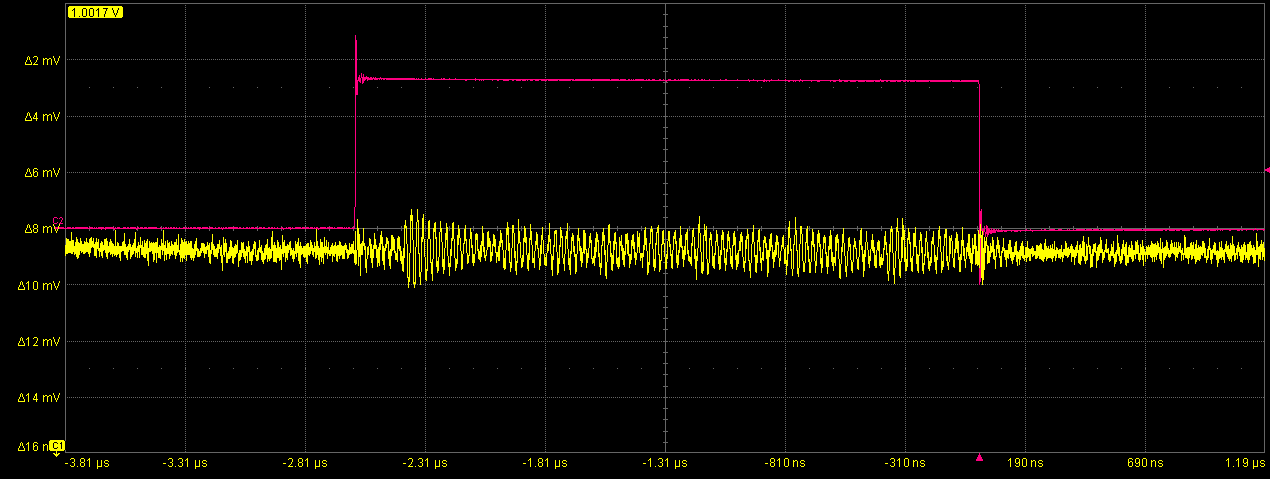
\includegraphics[scale=0.15]{report_pictures/snapstvla/sbox1_unmod1}
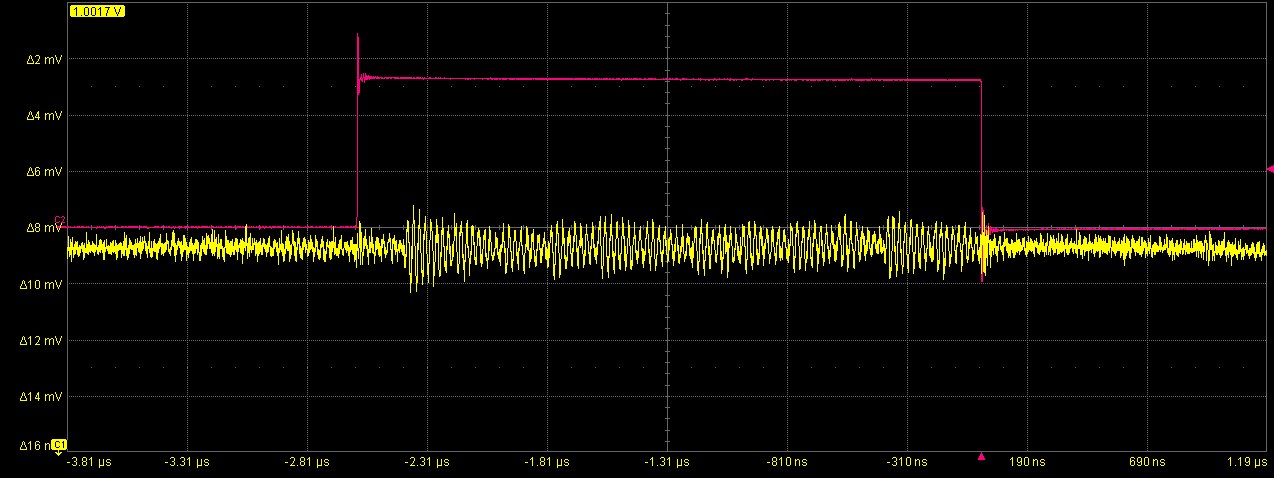
\includegraphics[scale=0.15]{report_pictures/snapstvla/sbox1_unmod2}
\par\end{centering}
\caption{Plots of two traces of LUT based AES to show how the plots change
for different inputs}

\end{figure}


\subsection{Composite Field Implementation}

As discussed earlier, here, we use composite field arithmetic to reduce
the byte-to-byte mapping to simpler operations. This allows for modifications
for side-channel resistance, and based on our previous research \cite{key-1},
we found it to occupy a lesser area. Our implementation of Forward
S-box uses only 39 LUTs. The rest of the modules for both Composite
Field and Lookup-table based implementations are the same.

In Composite Field theory, a higher dimension vector is projected
to components of vectors in the lower dimensions. We can then derive
efficient computations otherwise cumbersome in the original higher
dimension space. $GF(2^{8})$ involves expensive inverse multiplication
and can be reduced to inverse operations in $GF(2^{4})$. $GF(2^{4})$
can be further reduced to $GF(2^{2})$, but $GF(2^{4})$ is more suitable
for FPGAs for their 4/6-input LUTs and $GF(2^{2})$ operations are
more suited for ASICs. 

For our composite field $GF((2^{4})^{2})$ \cite{key-1}, these are
the irreducible polynomials used.
\begin{center}
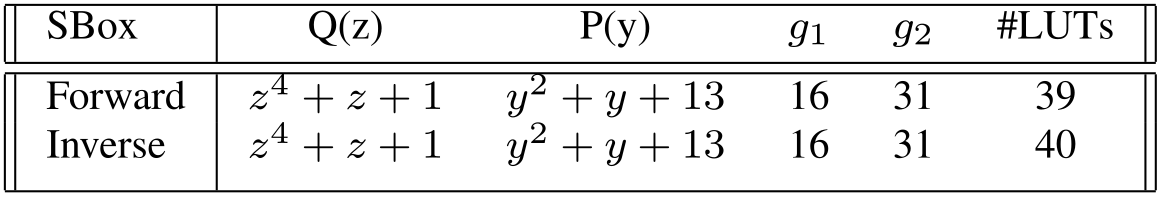
\includegraphics[scale=0.3]{report_pictures/pasted1}
\par\end{center}

where P(y) and Q(z) are the polynomials and g1, g2 are generators
for the composite and AES field.

We can see from the plots in Figure 4 how similar the traces are for
different inputs.

\begin{figure}[H]
\begin{centering}
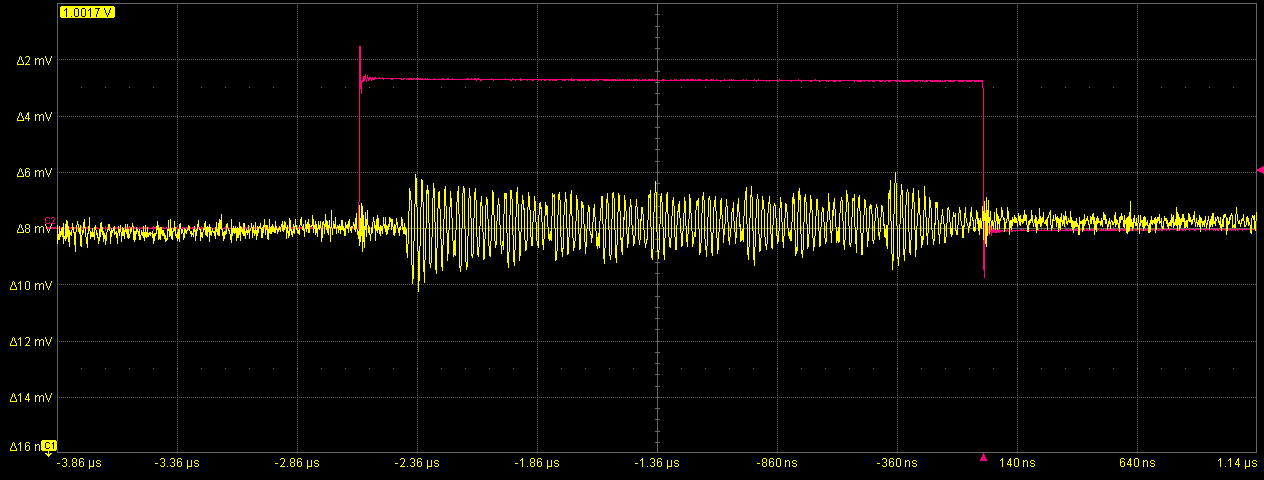
\includegraphics[scale=0.15]{report_pictures/snapstvla/sbox2_unmod}
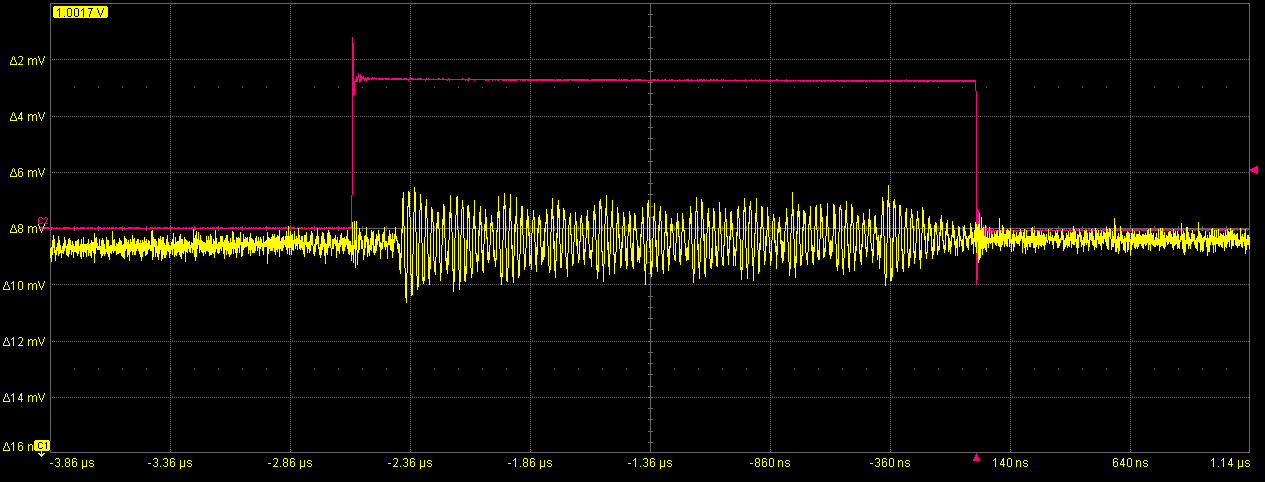
\includegraphics[scale=0.15]{report_pictures/snapstvla/sbox2_unmod2}
\par\end{centering}
\caption{Plots of two traces of Composite AES to show how the plots change
for different inputs}

\end{figure}

In the \emph{SubBytes} stage, the 128-bit text is split into 16 bytes
and each is fed into one S-box. S-boxes are also used in Key generation
modules. In our implementation, Key generation is done separately
before the cipher process as the same set of round keys are used for
all the processes. The main component of the 11 peaks in the power
trace is the 16 S-box transformations in each round.

\subsection{Threshold Implementation}

Threshold implementation \cite{key-11} of AES is built to ensure
more security of the S-box. Each input to the S-box, $X$, is split
across $n$ shares such that they follow the following property:

\noindent {\large{}
\begin{equation}
\sum_{i=1}^{n}X_{i}=X
\end{equation}
}{\large\par}

\noindent {\large{}
\begin{equation}
\sum_{i=1}^{n}F(X_{i})=F(X)=Y
\end{equation}
}{\large\par}

Additionally, even the output can be shared across $m$ shares which
sum up to give $Y$.

\noindent {\large{}
\begin{equation}
\sum_{i=1}^{m}Y_{i}=Y\:whereY_{i}=F_{i}(X_{1},X_{2},X_{3},...,X_{n})
\end{equation}
}{\large\par}

The function $F_{i}$ is identified such that it is independent of
the input $X_{i}$. This ensures that when each share is being executed
a particular $X$ component is not revealed. This uniform masking
makes the leaking signal almost a constant at all instants of time. 

Plots are added below in Figure 5, but it is difficult to differentiate
between them due to very low increase in power consumption. The low
power consumption is because only one S-box runs in a cycle. The S-box
for threshold implementation consumes more resources than the Composite
Field based S-box, and hence this strategy was followed.

\begin{figure}[H]
\begin{centering}
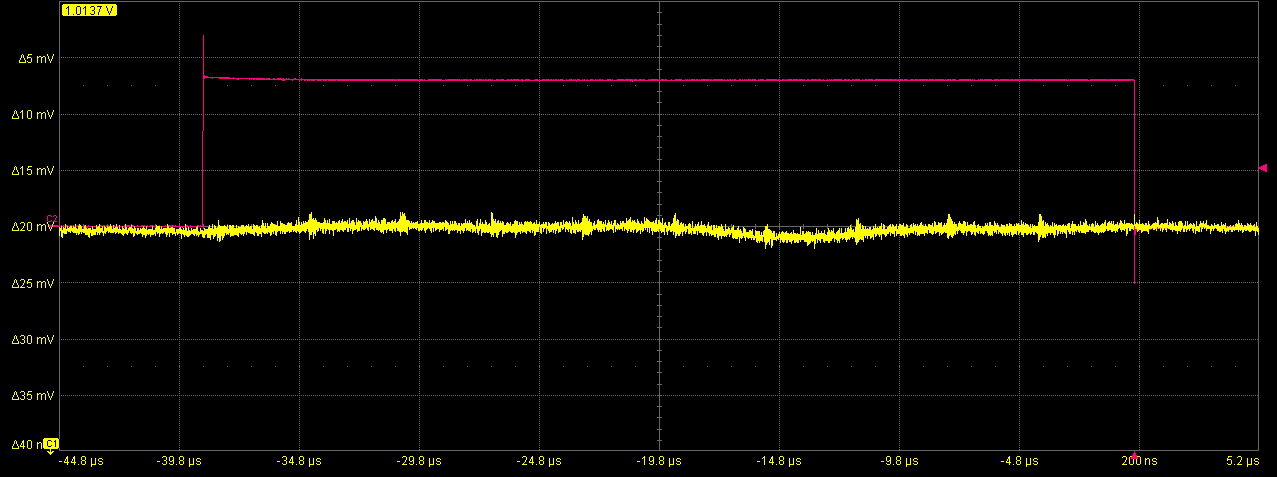
\includegraphics[scale=0.15]{report_pictures/snapstvla/thresh_unmod1}
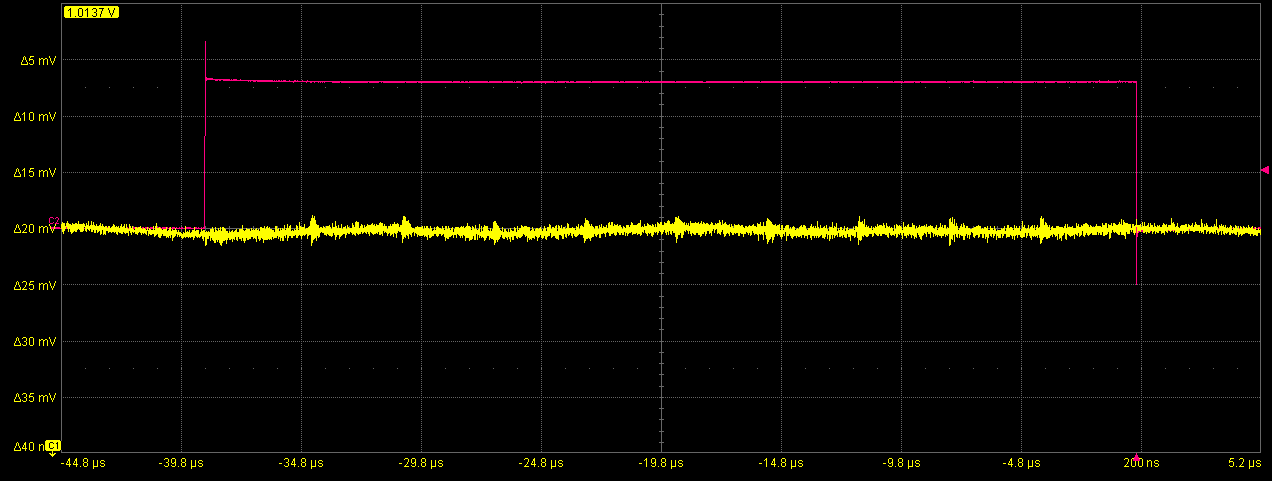
\includegraphics[scale=0.15]{report_pictures/snapstvla/thresh_unmod2}
\par\end{centering}
\caption{Plots of two traces of Threshold AES to show how the plots change
for different inputs}

\end{figure}


\subsection{Implementation details}

In this section, we briefly describe the implementation aspects of
the three accelerators. Among them, Lookup-table based and Composite
Field implementations use typical AES top modules while Threshold
implementatioon uses a different set of top modules. As discussed
earlier, the only difference between the the top modules is that the
typical version uses 16 S-boxes in parallel while the other uses only
one. Typical AES accelerator can be embedded with either LUT based
or Composite S-box.

The modules for typical AES accelerator have been modified for ease
of usage so that only the imported module needs to be changed to switch
between the S-box modules. The following figure shows the methods
of the top modules which are used for one cipher process. ``genKeys''
is used to initiate key generation, ``encrypt'' is used to pass
the plaintext for processing and ``ret'' returns the output of the
cipher process. Other methods are also present which can be used to
check the status of the process.

\begin{figure}[H]
\begin{centering}
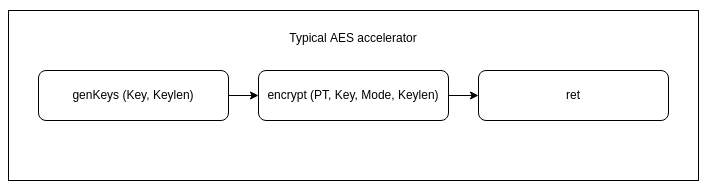
\includegraphics[scale=0.4]{report_pictures/typical_top}
\par\end{centering}
\caption{Flow diagram for Typical AES module}

\end{figure}

Threshold's top module is slightly different as here the ``encrypt''
method additionally checks if the Key received has been expanded before
and then continues with the cipher process.
\begin{figure}[H]
\begin{centering}
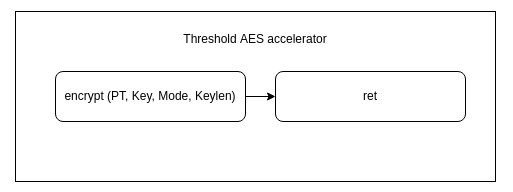
\includegraphics[scale=0.4]{report_pictures/thresh_top}
\par\end{centering}
\caption{Flow diagram for Threshold AES module}

\end{figure}
 

Following table sums up the different physical aspects of each implementation.
The hardware utilisations and maximum operable frequency of each accelerator
was found by implementing the accelerators on our FPGA. The wrapper
module used here is Wrapper2 and details about wrapper modules and
FPGA are discussed in the next section.

\begin{table}[H]
\noindent \centering{}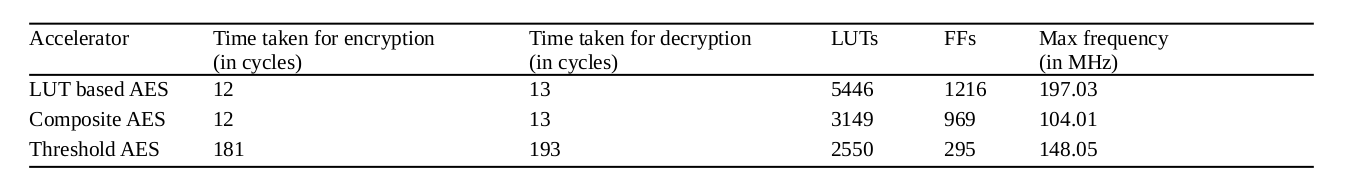
\includegraphics[scale=0.4]{report_pictures/acc_imp}
\end{table}

\pagebreak{}

\section{Side-channel evaluation of accelerators}
\noindent \begin{center}
This section covers the setup followed for the side-channel evaluation
of our AES accelerator. Similar procedure can be followed for other
accelerators too. The following are the steps involved:
\par\end{center}
\begin{itemize}
\item Make a wrapper module for the accelerators to feed the inputs to the
crypto-module
\item Configure the module for the FPGA with another Top file
\item Configure the oscilloscope as required and program the FPGA with our
module
\item Collect the traces and evaluate the TVLA score using Python scripts
\end{itemize}
We begin by making a wrapper module for the accelerators discussed
in the previous section. All the modules of the accelerator and wrapper
are written in Bluespec SystemVerilog and Verilog files are generated
from this. The top module for configuring the FPGA is written in Verilog
HDL.

Two wrapper modules were made using different approaches. For Wrapper1,
we have four stages as shown in Figure 8 and for Wrapper2, we have
five stages as shown in Figure 9. Details about the wrappers have
been given later.

We use the SASEBO-GIII board as the platform for evaluation and the
Teledyne LeCroy HDO4104 oscilloscope for collecting traces. After
that, the Python script is run to compute the TVLA score for each
set of traces. More details are provided in the following subsections.

\subsection{AES Wrapper modules}

There are multiple ways to pass the inputs, and we have chosen to
create a wrapper file for the accelerator to feed fixed and random
inputs to the core module. Random inputs are generated by feeding
the cipher output of the previous random input. This is in conformance
with NIST standards. We have made two variants to compare the effects:
in one (Wrapper1), the output of the encryption/decryption was stored
in a 128-bit register within the trigger along with other register
updates, and in the other (Wrapper2), the total number of flip-flop
changes in the wrapper module was limited to 2 bits within the trigger.

\begin{figure}[H]
\begin{centering}
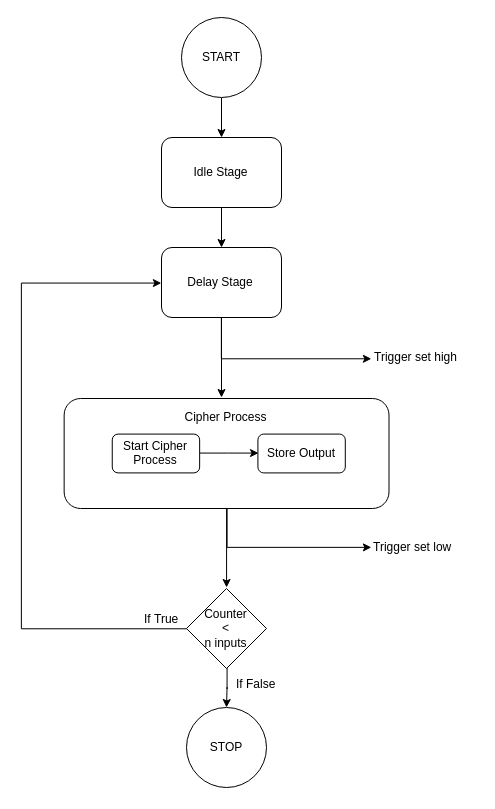
\includegraphics[scale=0.35]{report_pictures/wrapper1}
\par\end{centering}
\caption{Working of Wrapper1 module }

\end{figure}

As can be seen from Figure 8, Wrapper1 is a simple module with four
stages and three of them repeating till n inputs have been fed. The
delay stage is very crucial as the oscilloscope needs some time between
two traces to properly store the power values. In Figure 9, the working
of Wrapper2 module is shown and the main difference is that the cipher
process is repeated twice.

\begin{figure}[H]
\begin{centering}
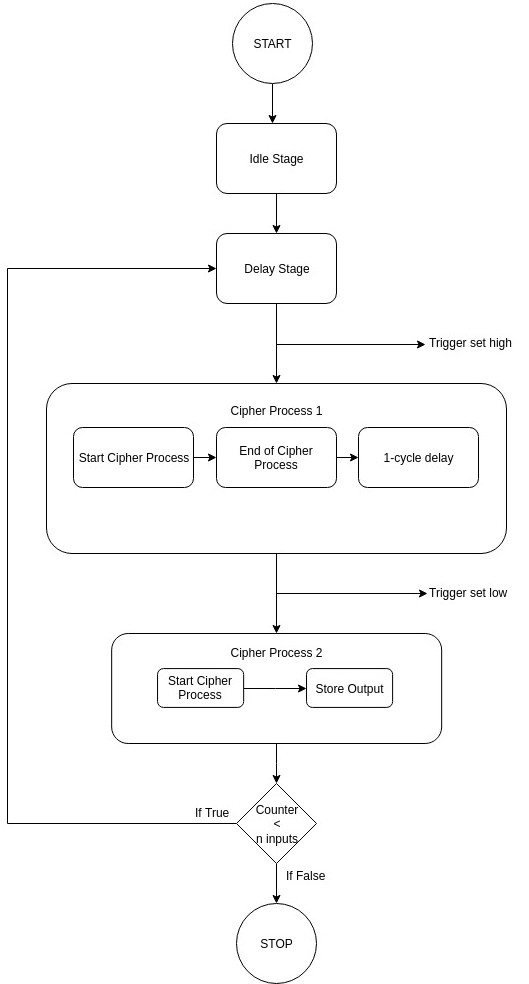
\includegraphics[scale=0.35]{report_pictures/wrapper2}
\par\end{centering}
\caption{Working of Wrapper2 module}

\end{figure}


\subsection{SASEBO-GIII board}

The SASEBO-GIII is a successor of the SASEBO-GII board and is for
further side-channel attack experimentation. The basic features of
SASEBO-GIII are as follows:
\begin{itemize}
\item 200 mm x 150 mm x 1.6mm, FR-4, eight layers
\item Two Xilinx FPGAs:
\begin{itemize}
\item Cryptographic FPGA: Kintex-7 XC7K160T-1FBGC (part no.: xc7k160tfbg676-1) 
\item Control FPGA: Spartan-6 XC6LX45-2FGG484C
\end{itemize}
\item Differential clock at frequency of 200 Mhz.
\item 1 Gigabit DDR3 SDRAM
\item The external power source supplies the onboard power regulators and
the FPGAs with 5.0 V
\item A shunt resistor is provided to insert on the core VDD line of the
cryptographic FPGA for measuring power traces. 
\end{itemize}
The host PC controls and communicates with the board via the J-TAG
port. The FPGA is default programmed with the vendor's Bit file. The
default Bit file can be found on the company's website and can be
used to collect traces using the C\# project, SASEBO G-CHECKER. 

For this project, Xilinx Vivado 2020.1 was used to program the Kintex-7
FPGA with our AES accelerator. The SASEBO Board uses a differential
clock and it needs to be converted into single-ended clock using a
clock wizard. In Vivado 2020.1, it can be found as the Xilinx IP,
clk\_wizard. The single-ended clock can be configured for frequencies
from 4.7 MHz to 800 MHz. Differential clocks have the advantage that
it is based on the difference between two signals and are less affected
by noise, and require lower supply voltages. 

\begin{figure}[H]
\begin{centering}
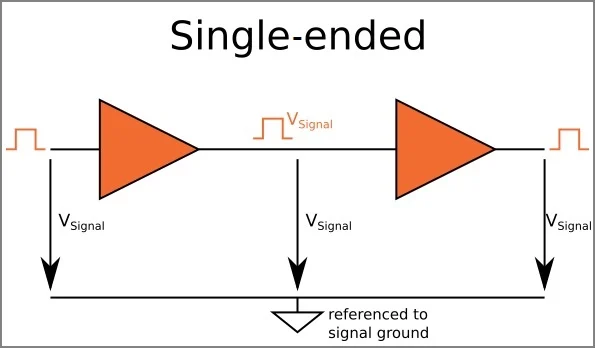
\includegraphics[scale=0.4]{report_pictures/single_ended} 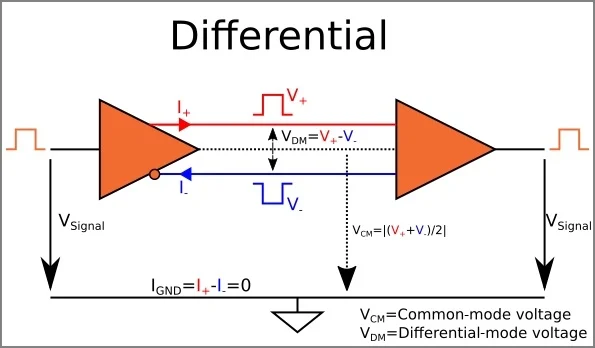
\includegraphics[scale=0.4]{report_pictures/differential}
\par\end{centering}
\caption{Distinctions between a single-ended and differential clock}

\end{figure}


\subsection{Oscilloscope}

Teledyne LeCroy HDO4104 was used for collecting the power traces from
the FPGA. Important features of this oscilloscope are as follows:
\begin{itemize}
\item Bandwidth of $1GHz$ 
\item Maximum sampling rate of $2.5GS/s$ 
\item Resolution of 12 bits
\item Four input channels
\item Processor/CPU - Intel Celeron B810 Dual-Core, 1.6GHz
\item Memory of 4GB RAM and 500GB disk
\item Oscilloscope Operating Software - Teledyne LeCroy MAUI with OneTouch
\end{itemize}
Other features also exist, such as trigger types, filters for analysis
and remote control setup. The oscilloscope uses an initial setup file,
aes-initial-verilog-{}-00000.lss. This uses default configurations
and sets all the system variables.

For collecting traces, both C1 and C2 channels are used. C1 is connected
to the measuring port of the FPGA and C2 collects the trigger signal
from the board pins. Data is collected whenever the trigger is set
high. We use a power probe for C1 and a single hook probe for C2.

We set the sampling rate to $10kS$, which is the number of samples
to be collected in each trigger. This is not achievable in case of
the typical AES accelerator (non-threshold AES), and instead, the
oscilloscope will reduce the sampling rate on its own to around 5000-6000
samples per trigger based on the resolution. The sample size will
be fixed for all traces provided we ensure in our design that the
trigger is set for the same number of cycles for each trace. The oscilloscope
can also synchronise triggers to give a clear and stable display of
the power traces.

\subsection{Code analysis of Python scripts}

After collecting the traces, the python code TVLA\_threaded.py can
be used to compute the TVLA score. This code involves multithreading,
and a corresponding sequential code was also made and can be found
as TVLA\_basic.py. The scores from the two codes differ only by 0.001\%
which is occuring due to floating point precision errors.

\subsubsection{Libraries imported}

The following libraries are imported:

\begin{lstlisting}
import os
import pandas as pd
import numpy as np
import csv
import threading as th
from time import time
from joblib import Parallel, delayed
\end{lstlisting}


\subsubsection{TVLA\_basic.py}

TVLA\_basic.py is a simple sequential code that can read a file iteratively
and accumulate the total sum and sum of squares for mean and variance
computation. Power consumption at each instant of time is present
in consecutive rows, and the t-value is found for each row separately.
The following summations were used so that all the trace files need
not be read and stored together for processing. This was done to prevent
RAM from getting full and to also allow parallel processing of data
which we utilize in the next script.

\noindent {\large{}
\begin{equation}
Mean_{j}(\mu_{j})=\frac{1}{N}\sum_{k=1}^{N}row_{k}[j]
\end{equation}
}{\large\par}

\noindent {\large{}
\begin{equation}
Variance_{j}(\sigma_{j})=\frac{1}{N}(\sum_{k=1}^{N}row_{k}[j]^{2})-\mu_{j}^{2}
\end{equation}
}{\large\par}
\noindent \begin{center}
where N is the number of traces, k is the kth trace and j is jth instant
of time during the trigger
\par\end{center}

This computation is done separately for dataset 1 and dataset 2. T-value
is computed at every time instant, and the highest value is displayed
in the end along with the time taken.

\subsubsection{TVLA\_threaded.py}

This code is similar to the previous one but with the added advantage
of threads. Threads are lightweight processes and allow parallel processing
of data. If we are to use threads, we should try to ensure that the
number of threads getting generated is some multiple of the number
of cores we are using so that we get maximum efficiency. Threads are
introduced using the Joblibs library.

To compute the total sum and sum of squares, we use reduction sum
approach. This was found to be significantly faster than each thread
returning values reading from a file. A function, \emph{partial\_accumulator()},
is defined which takes the parameters \emph{csv\_files}, loop variable
\emph{i}, \emph{width} and number of traces. Using \emph{Parallel()},
we generate threads, and each will perform this function.

We use a parameter ``\emph{width}'' for which each thread will compute
the partial sums. For good efficiency, the total number of traces
by \emph{width} should be a multiple of the number of cores. Other
parameter in this code is the number of cores which ideally should
be the number of cores in the computing system used.

\section{Evaluation of AES accelerators}

Both encryption and decryption processes were evaluated in separate
experiments for each of our AES accelerators. For the TVLA test, two
sets of data \cite{key-6} are to be passed by the Wrapper modules
for both encryption and decryption.
\begin{enumerate}
\item Data-set 1:
\begin{enumerate}
\item 256-bit Constant Key is set to 0x0123456789abcdef123456789abcdef023456789abcdef013456789abcdef012
and Key length is set to Bit128
\item $n$ 128-bit fixed input is set to 0xda39a3ee5e6b4b0d3255bfef95601890
where $n$ is the number of times the fixed input is fed
\end{enumerate}
\item Data-set 2:
\begin{enumerate}
\item 256-bit Constant Key is set to 0x0123456789abcdef123456789abcdef023456789abcdef013456789abcdef012
and Key length is set to Bit128
\item $n$ 128-bit inputs: $I_{0}$, $I_{1}$, ..., $I_{n}$, where $I_{0}=0x0$,
$I_{j}=AES(Key,I_{j},mode)$ for $0<j\leq n$ where $n$ is the number
of inputs and mode is for choosing between encryption and decryption
\end{enumerate}
\end{enumerate}
As it can be noted, the same Key is used for both the datasets and
the same number of inputs were fed for both the datasets. NIST recommends
dispersing the two datasets while emulating them, so we passed the
inputs from both the datasets alternatively. We use only Kintex7 (part
no.: xc7k160tfbg676-1) of the SASEBO-GIII board, and it was programmed
using Xilinx Vivado 2020.1. 

The following picture is the setup used for the above three accelerators.
\begin{center}
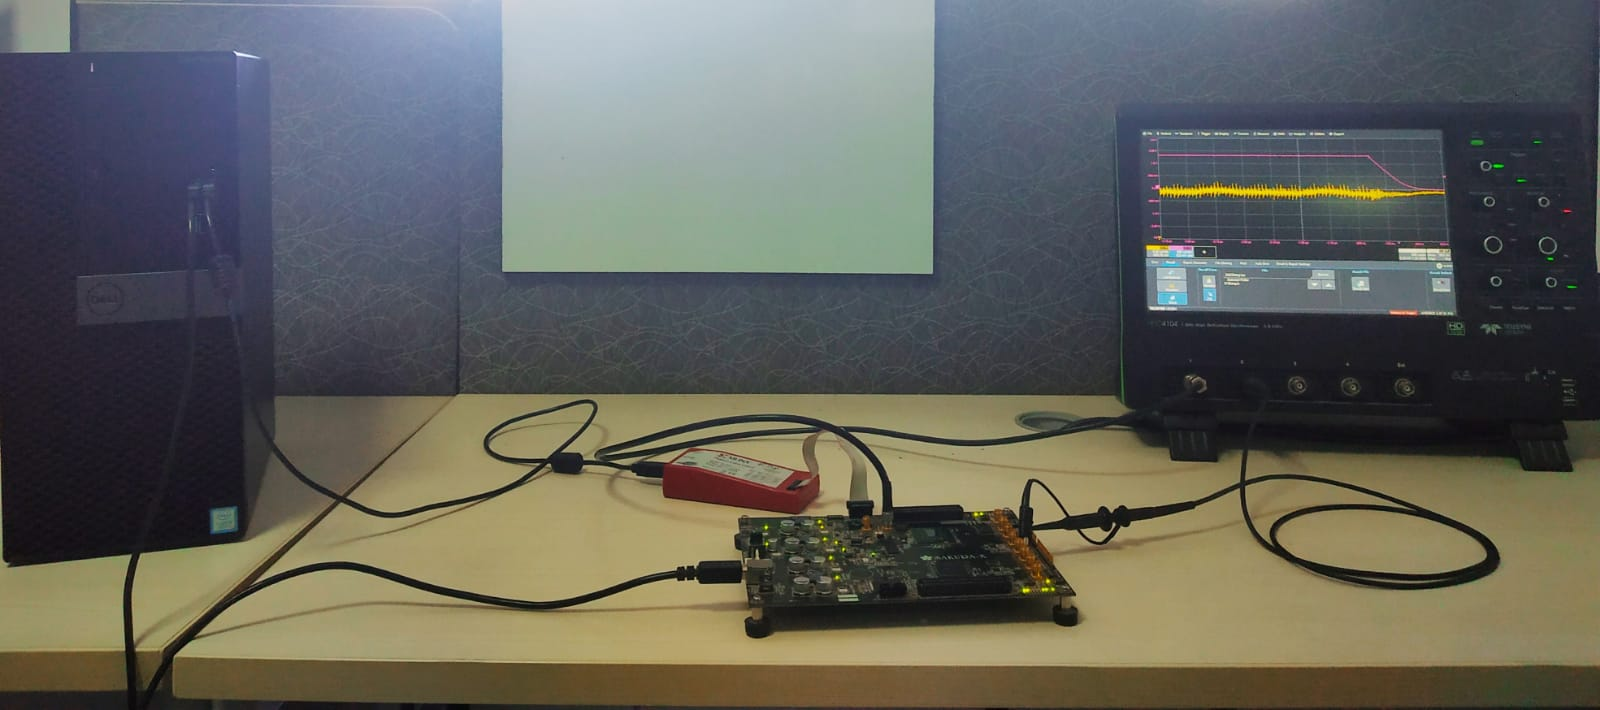
\includegraphics[scale=0.2]{report_pictures/setup}
\par\end{center}

Two connections were given from the FPGA to the oscilloscope, as shown
in the above picture. C1 of the oscilloscope is connected to the power
measuring port, and C2 of the oscilloscope collects the trigger signal
from the board's pins. The Xilinx Platform Cable connects to the FPGA
via the JTAG interface and is used for programming the FPGA using
Vivado. 

To feed the inputs to the accelerators we use wrapper modules. The
wrapper files have the following ports:

\begin{lstlisting}
input  CLK;
input  RST_N;

// value method trigger_pin
output trigger_pin;

// value method done_signal
output done_signal;

// value method output_fix
output [127 : 0] output_fix;
\end{lstlisting}

In the Top module above the wrapper file, we have given just the minimum
required configurations required for the FPGA. To convert the differential
clock of the FPGA to a single-ended clock, we added a Xilinx IP, clk\_wizard.
This will be present in the Top module which is written in Verilog
HDL. The input frequency needs to be set to the SASEBO board's frequency
of 200MHz, and the output frequency was set to 5MHz. Reset is set
as active high.

\begin{figure}[H]
\begin{centering}
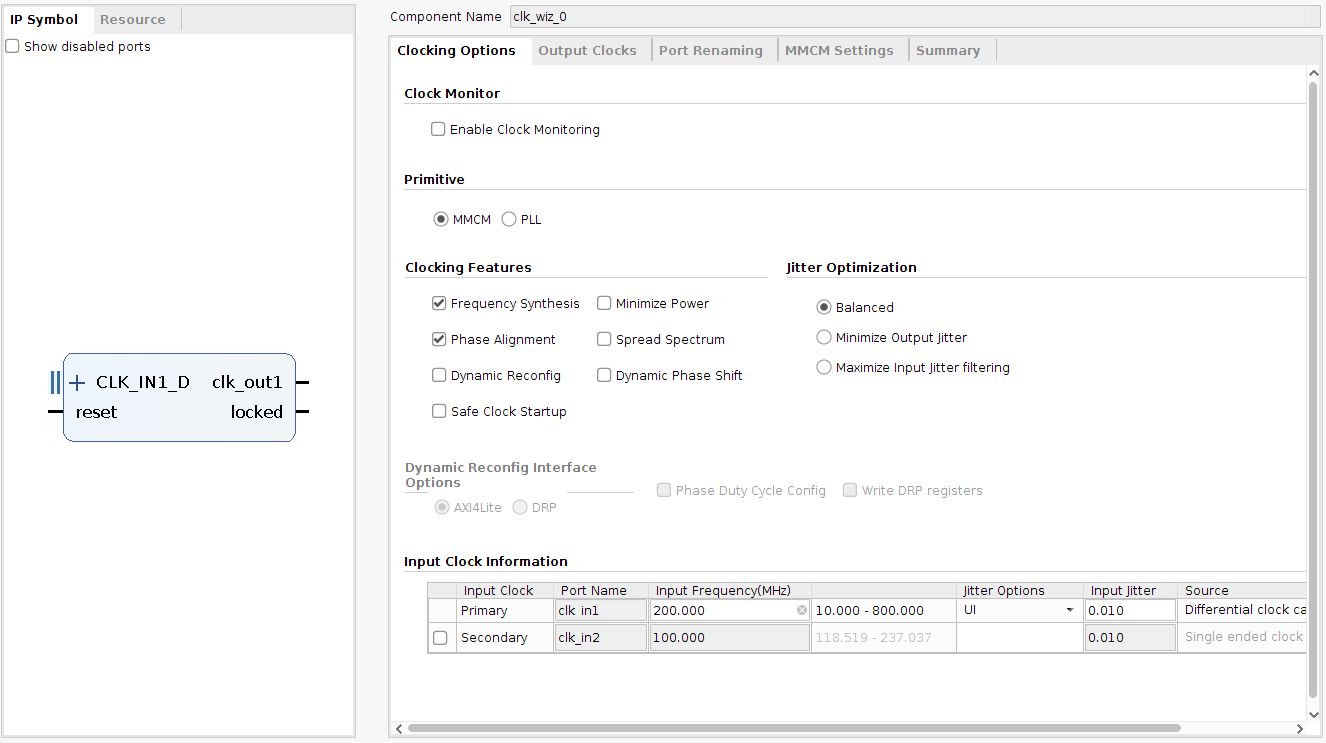
\includegraphics[scale=0.2]{report_pictures/clk_wiz1}$\:$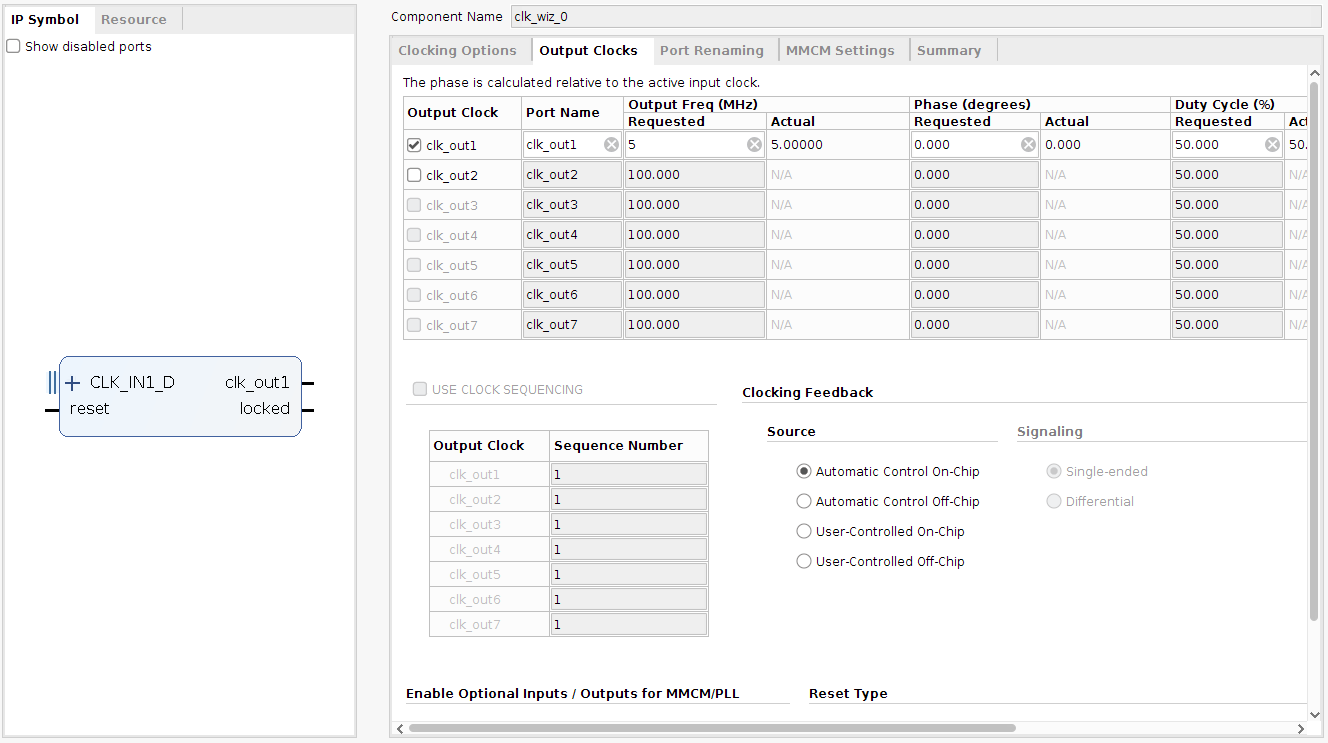
\includegraphics[scale=0.2]{report_pictures/clk_wiz2}
\par\end{centering}
\caption{Clk\_wizard configuration}

\end{figure}

The following constraint file was used for the FPGA. Vivado's default
settings were used for synthesis and implementation.

\begin{lstlisting}
## Clock configuration
set_property -dict {PACKAGE_PIN AA3 IOSTANDARD LVDS} [get_ports CLK_P] 
set_property -dict {PACKAGE_PIN AA2 IOSTANDARD LVDS} [get_ports CLK_N]

## RESET configuration
set_property -dict {PACKAGE_PIN L23 IOSTANDARD LVCMOS25} [get_ports RST_N]

## GPIO configuration
set_property -dict {PACKAGE_PIN E23 IOSTANDARD LVCMOS25} [get_ports gpio0]
set_property -dict {PACKAGE_PIN N17 IOSTANDARD LVCMOS25} [get_ports gpio1]
set_property -dict {PACKAGE_PIN P24 IOSTANDARD LVCMOS25} [get_ports gpio2]

# General configuration
set_property BITSTREAM.General.UnconstrainedPins {Allow} [current_design]
\end{lstlisting}

The oscilloscope is set to sample $10kS$ points for each trigger,
and the trigger mode is set to window trigger. For the proper collection
of traces, a large delay of 600ms is given between two traces in the
Wrapper module. This is about the time required for the oscilloscope
to save the collected data before sampling the next one. The approximate
time taken to collect $50K$ traces is 8 hours. After generating traces,
it is suggested to move the files from one device to another in a
zip folder to prevent any data loss during transfer. After collecting
the data, we unzip the folder and set the appropriate parameters in
the python script and execute the code.

\pagebreak{}

\subsection{Evaluation of Lookup-table Based Implementation}

For the typical AES accelerator with LUT based S-box, 25,000 inputs
were given from each dataset. We perform four tests: encryption process
with both the wrappers and decryption process for both the wrappers.
The number of clock cycles one process takes is 12 for encryption
and 13 for decryption and the FPGA's frequency is set at 5 MHz. Using
our Teledyne Lecroy oscilloscope we set the maximum sampling rate
at 10K samples per trigger. We set the oscilloscope to resolution
of $2mV/div$ and $500ns/div$. For the python script, the number
of cores is set to $10$ and the width is set to $1000$. The following
table depicts the implementation details for comparing the two wrapper
modules.
\begin{center}
\begin{table}[H]
\noindent \centering{}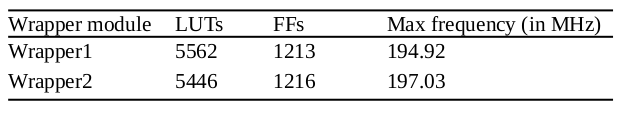
\includegraphics[scale=0.4]{report_pictures/LUT}
\end{table}
\par\end{center}

\subsubsection*{Evaluation with Wrapper1}

Following plots are the TVLA plots for encryption and decryption process
using Wrapper1. The sampling rate was at 5001 samples per trigger
for both the processes. Note that the x-axis is in sample units.
\noindent \begin{center}
\begin{figure}[H]
\noindent \centering{}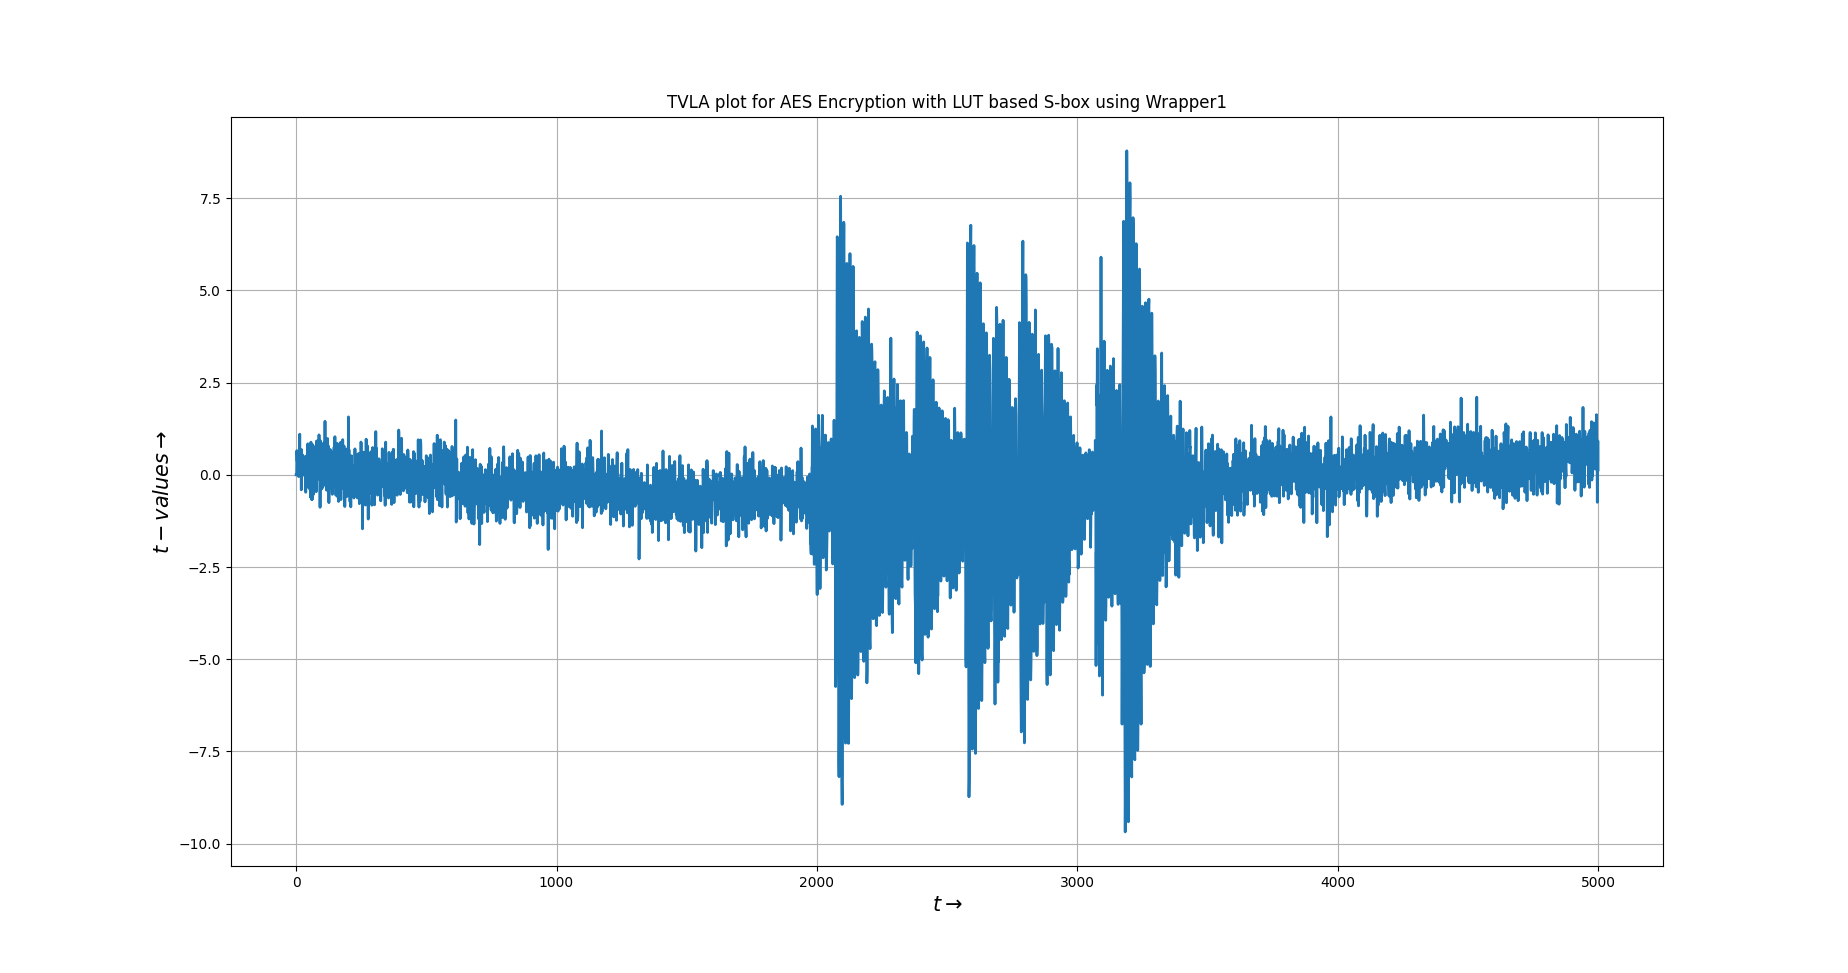
\includegraphics[scale=0.35]{report_pictures/temp_pics/Figure_1b}
\end{figure}
\par\end{center}

\begin{figure}[H]
\begin{centering}
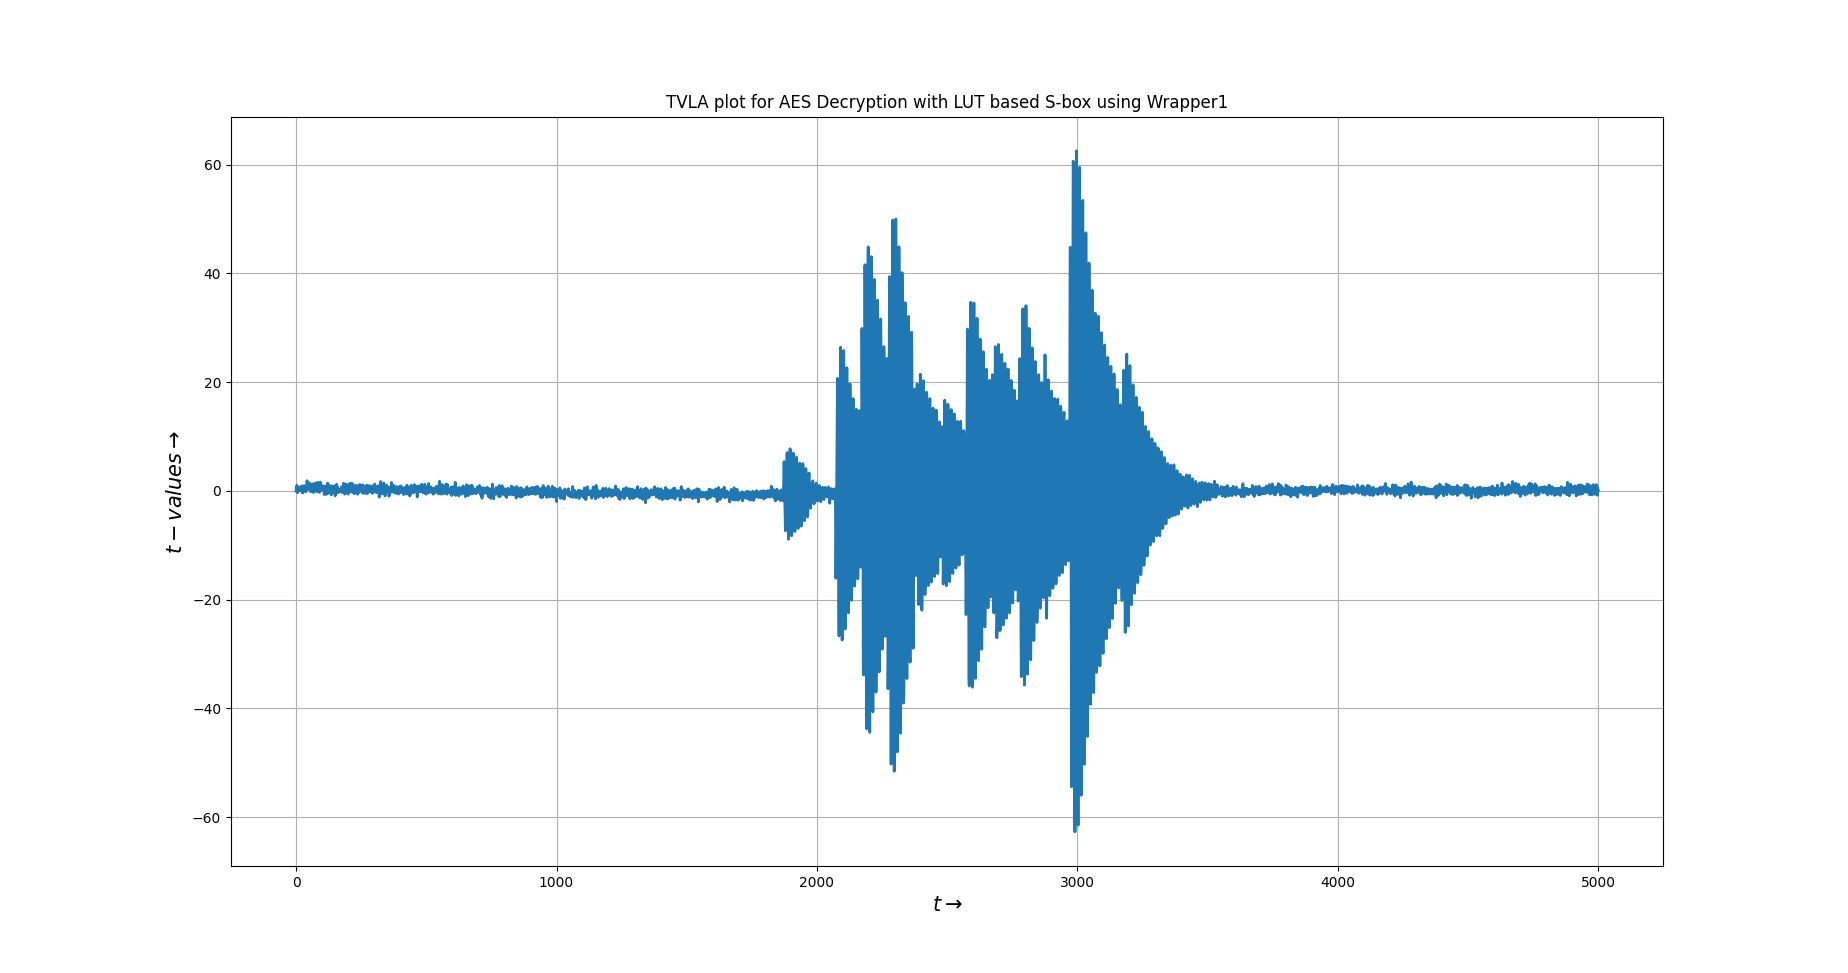
\includegraphics[scale=0.35]{report_pictures/temp_pics/Figure_4b}
\par\end{centering}
\caption{Plots for Encryption and Decryption process for LUT based S-box with
Wrapper1}
\end{figure}

The same starting random input, $0x00$, was used for both the tests.
We have also calculated the TVLA score for different number of traces. 

\begin{table}[H]
\caption{TVLA scores for encryption with LUT based S-box using Wrapper1}

\noindent \centering{}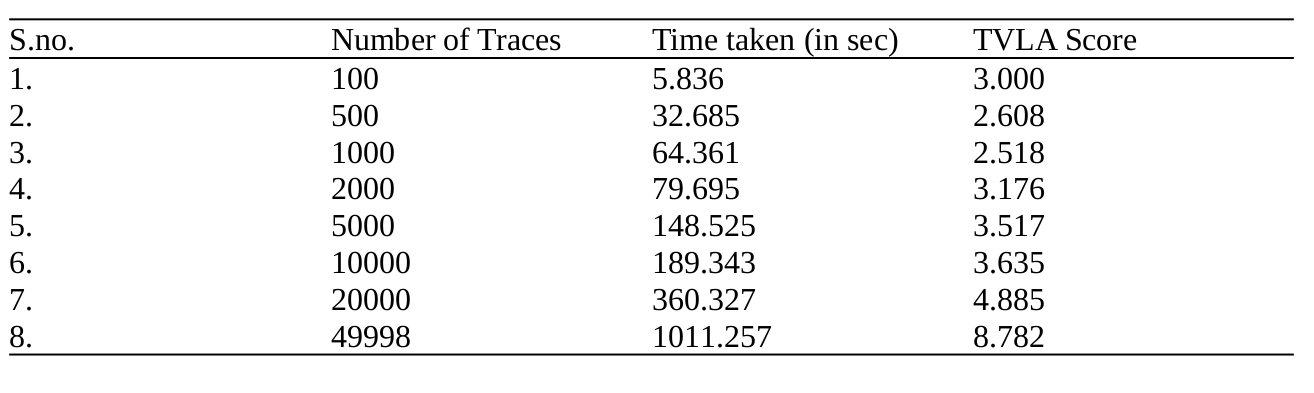
\includegraphics[scale=0.4]{report_pictures/temp}
\end{table}

\begin{table}[H]
\caption{TVLA scores for decryption with LUT based S-box using Wrapper1}

\centering{}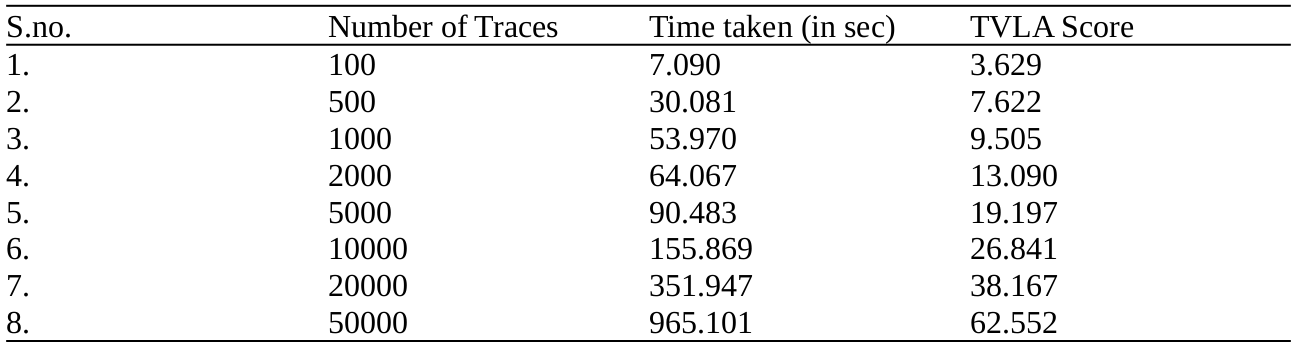
\includegraphics[scale=0.4]{report_pictures/sbox1_decr_w1}
\end{table}

\pagebreak{}

Additionally, we have run the TVLA scripts for different width (same
number of cores) to see which is the most efficient. For this only
one set of data with 50K traces, traces for encryption with LUT based
S-box using Wrapper1, was used. Due to optimizations in the memory
access patterns, the time taken values in Table 5 are smaller than
in Table 3.

\begin{table}[H]
\caption{Analysis of width vs time taken for 50K traces}

\centering{}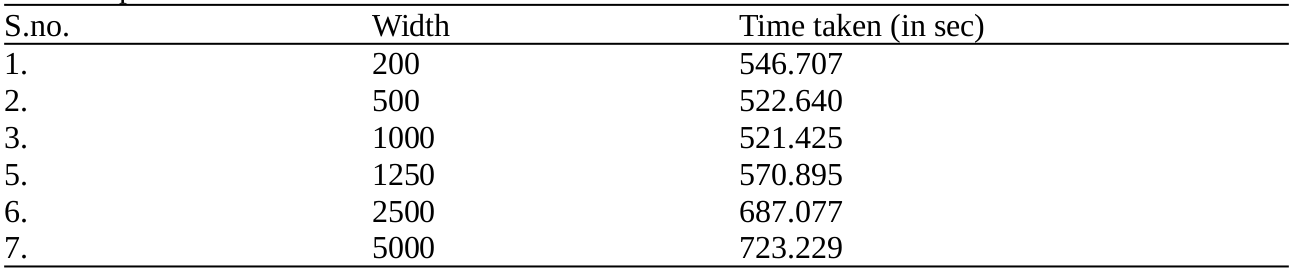
\includegraphics[scale=0.4]{report_pictures/time_50k}
\end{table}


\subsubsection*{Evaluation with Wrapper2}

Following plots are the TVLA plots for encryption and decryption process
using Wrapper2. The sampling rate was at 5001 and 10001 samples per
trigger for encryption and decryption process respectively. 
\begin{center}
\begin{figure}[H]
\centering{}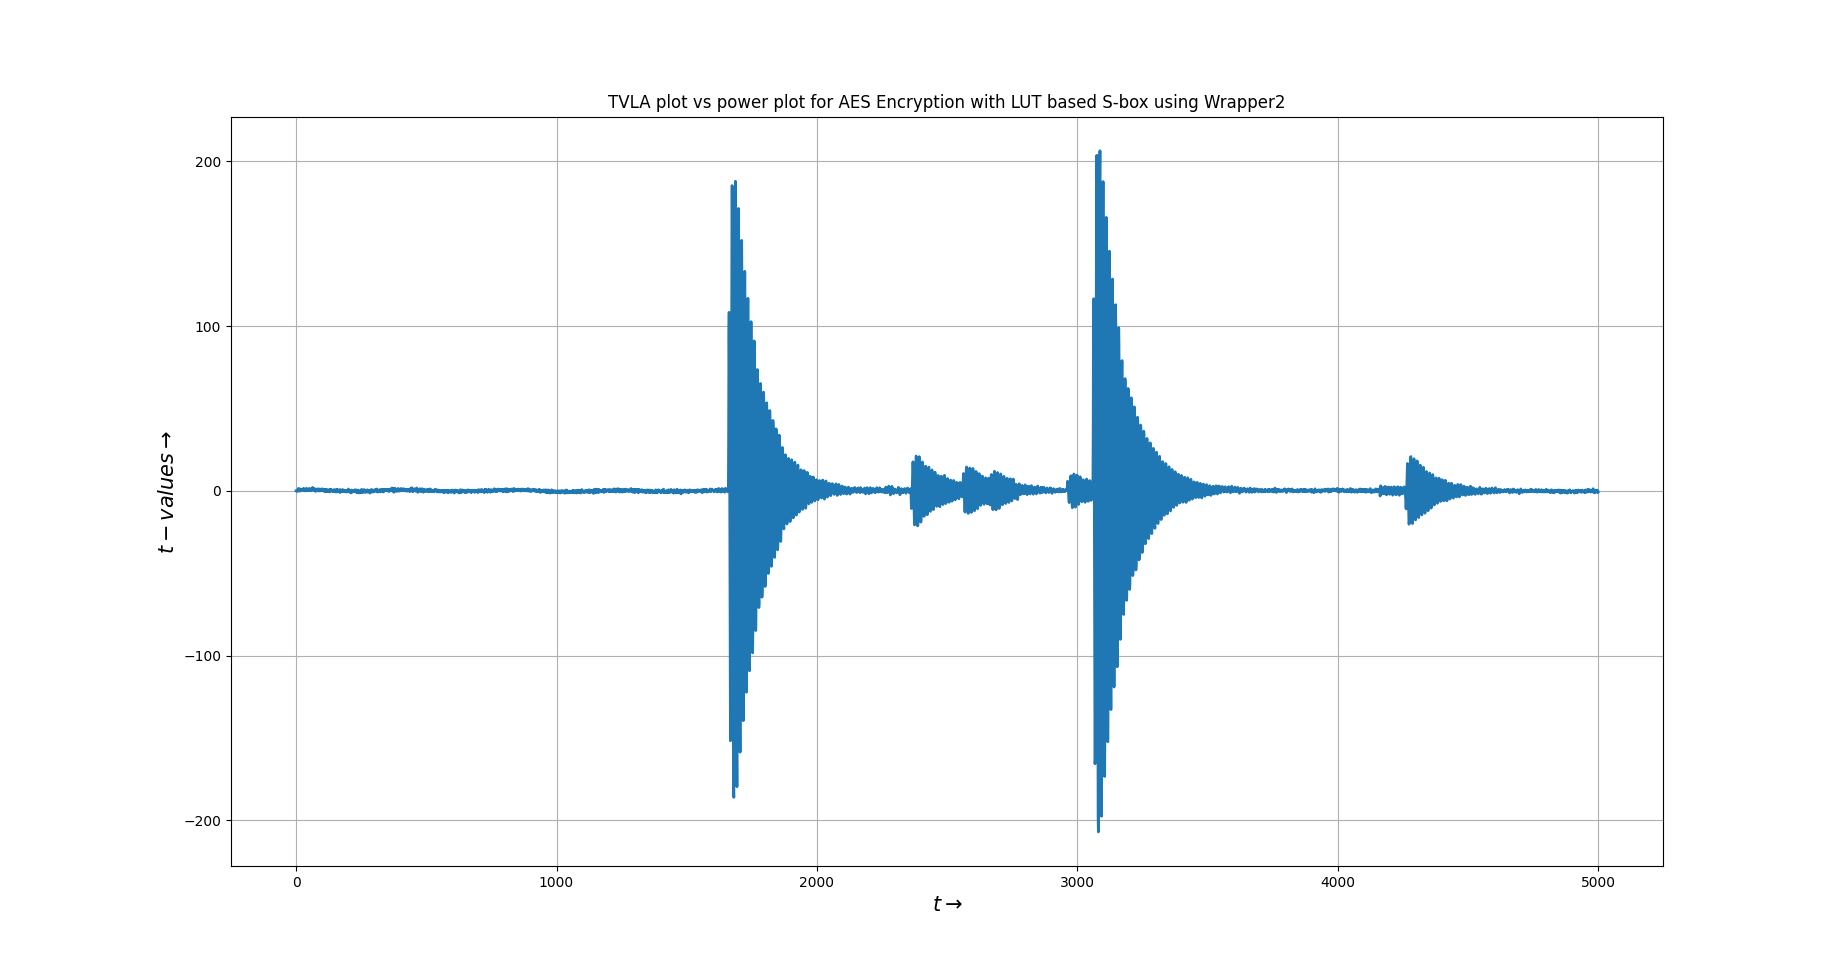
\includegraphics[scale=0.35]{report_pictures/temp_pics/Figure_3b}
\end{figure}
\par\end{center}

\begin{figure}[H]
\begin{centering}
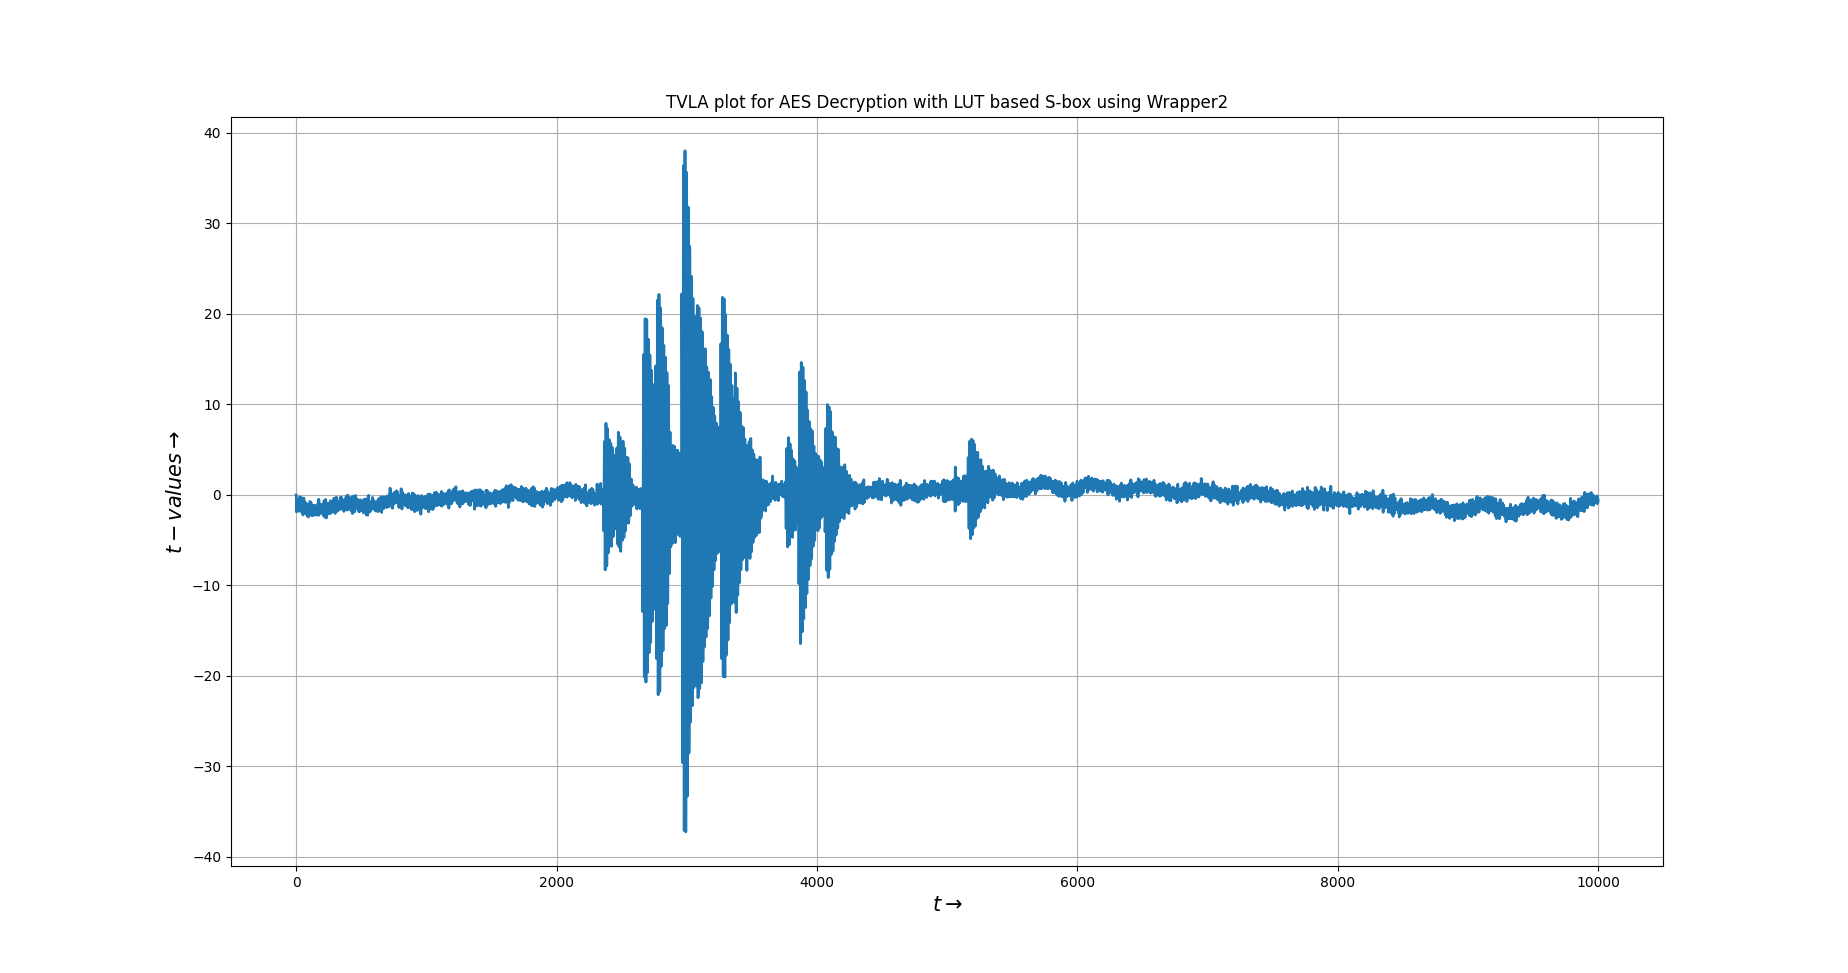
\includegraphics[scale=0.35]{report_pictures/temp_pics/Figure_7b}
\par\end{centering}
\caption{Plots for Encryption and Decryption process for LUT based S-box with
Wrapper2}

\end{figure}

Similar to previous, the same starting random input, $0x00$, was
used for both the tests and TVLA score was calculated for different
number of traces.

\begin{table}[H]
\caption{TVLA scores for encryption with LUT based S-box using Wrapper2}

\centering{}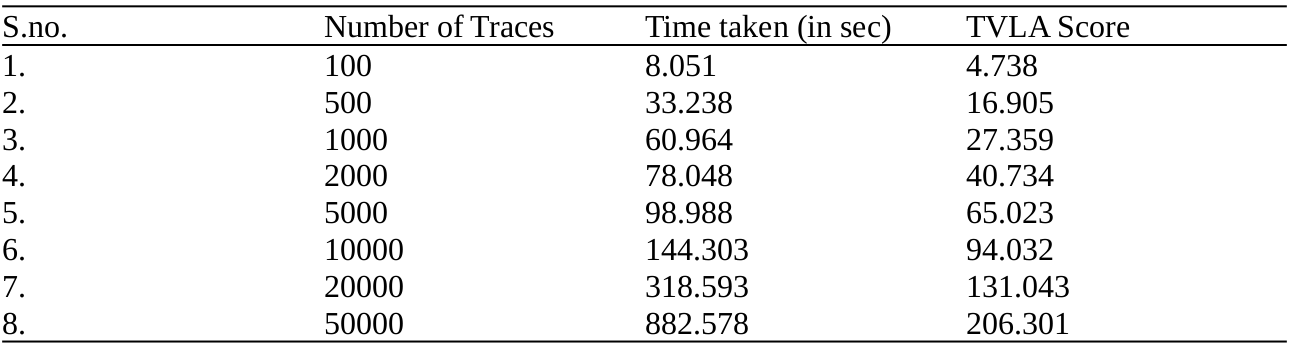
\includegraphics[scale=0.4]{report_pictures/sbox1_encr_w2}
\end{table}

\begin{table}[H]
\caption{TVLA scores for decryption with LUT based S-box using Wrapper2}

\centering{}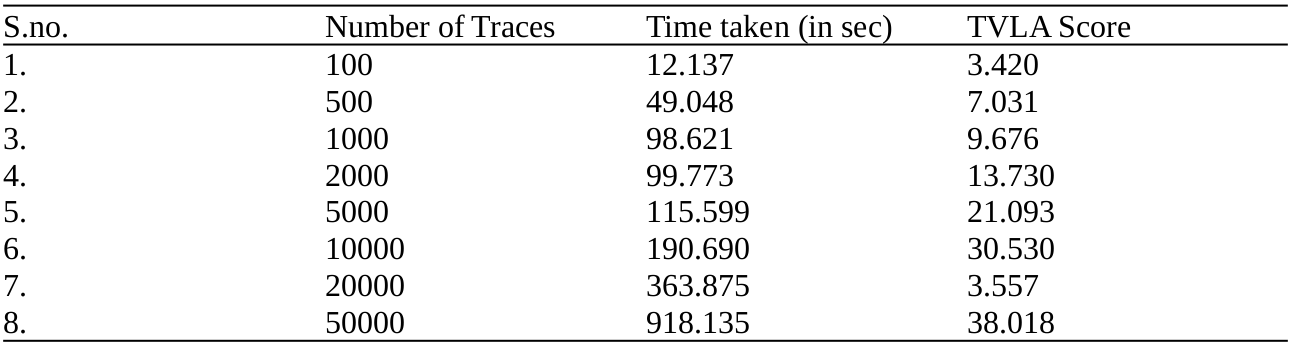
\includegraphics[scale=0.4]{report_pictures/sbox1_decr_w2}
\end{table}

Time analysis of workload for each thread is not done for these datasets
as it gave similar results as the previous one.

\subsection{Evaluation of Composite Field Implementation}

For the typical AES accelerator with Composite S-box too, we give
25,000 inputs from each dataset and separately conduct four tests
for encryption and decryption processes with both the wrappers. This
also takes the same number clock cycles as the previous. Using our
Teledyne Lecroy oscilloscope we set the maximum sampling rate at 10K
samples per trigger. We set the oscilloscope to resolution of $2mV/div$
and $500ns/div$. For the python script, the number of cores is set
to $10$ and the width is set to $1000$. The following table depicts
the implementation details for comparing the two wrapper modules.

\begin{table}[H]
\centering{}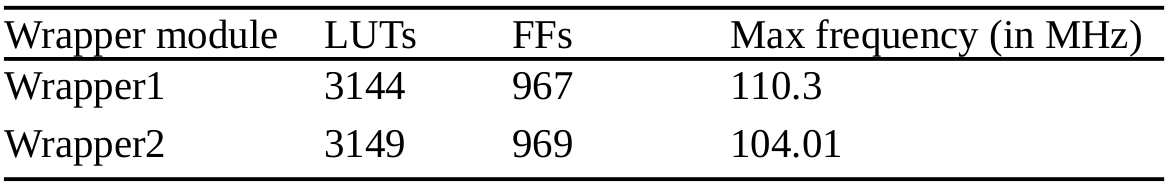
\includegraphics[scale=0.25]{report_pictures/Composite}
\end{table}


\subsubsection*{Evaluation with Wrapper1}

Following plots are the TVLA plots for encryption and decryption process
using Wrapper1. The sampling rate was at 5001 samples per trigger
for both the processes.
\begin{center}
\begin{figure}[H]
\centering{}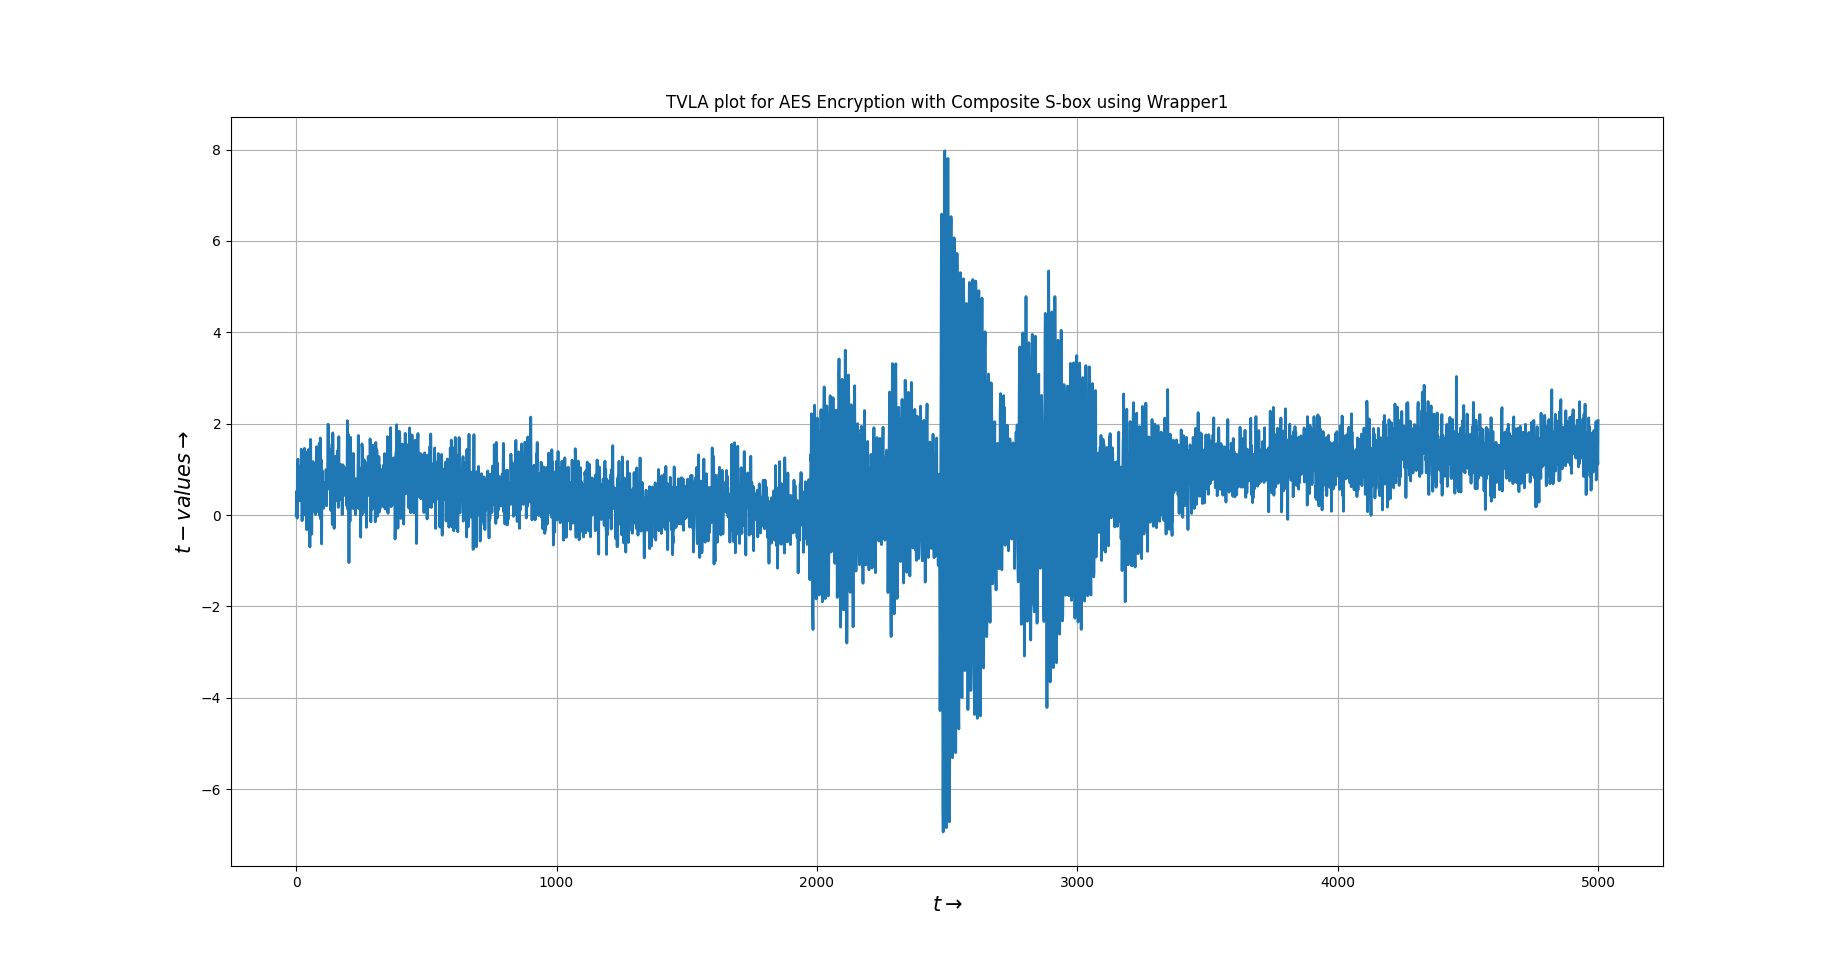
\includegraphics[scale=0.35]{report_pictures/temp_pics/Figure_8b}
\end{figure}
\par\end{center}

\begin{figure}[H]
\begin{centering}
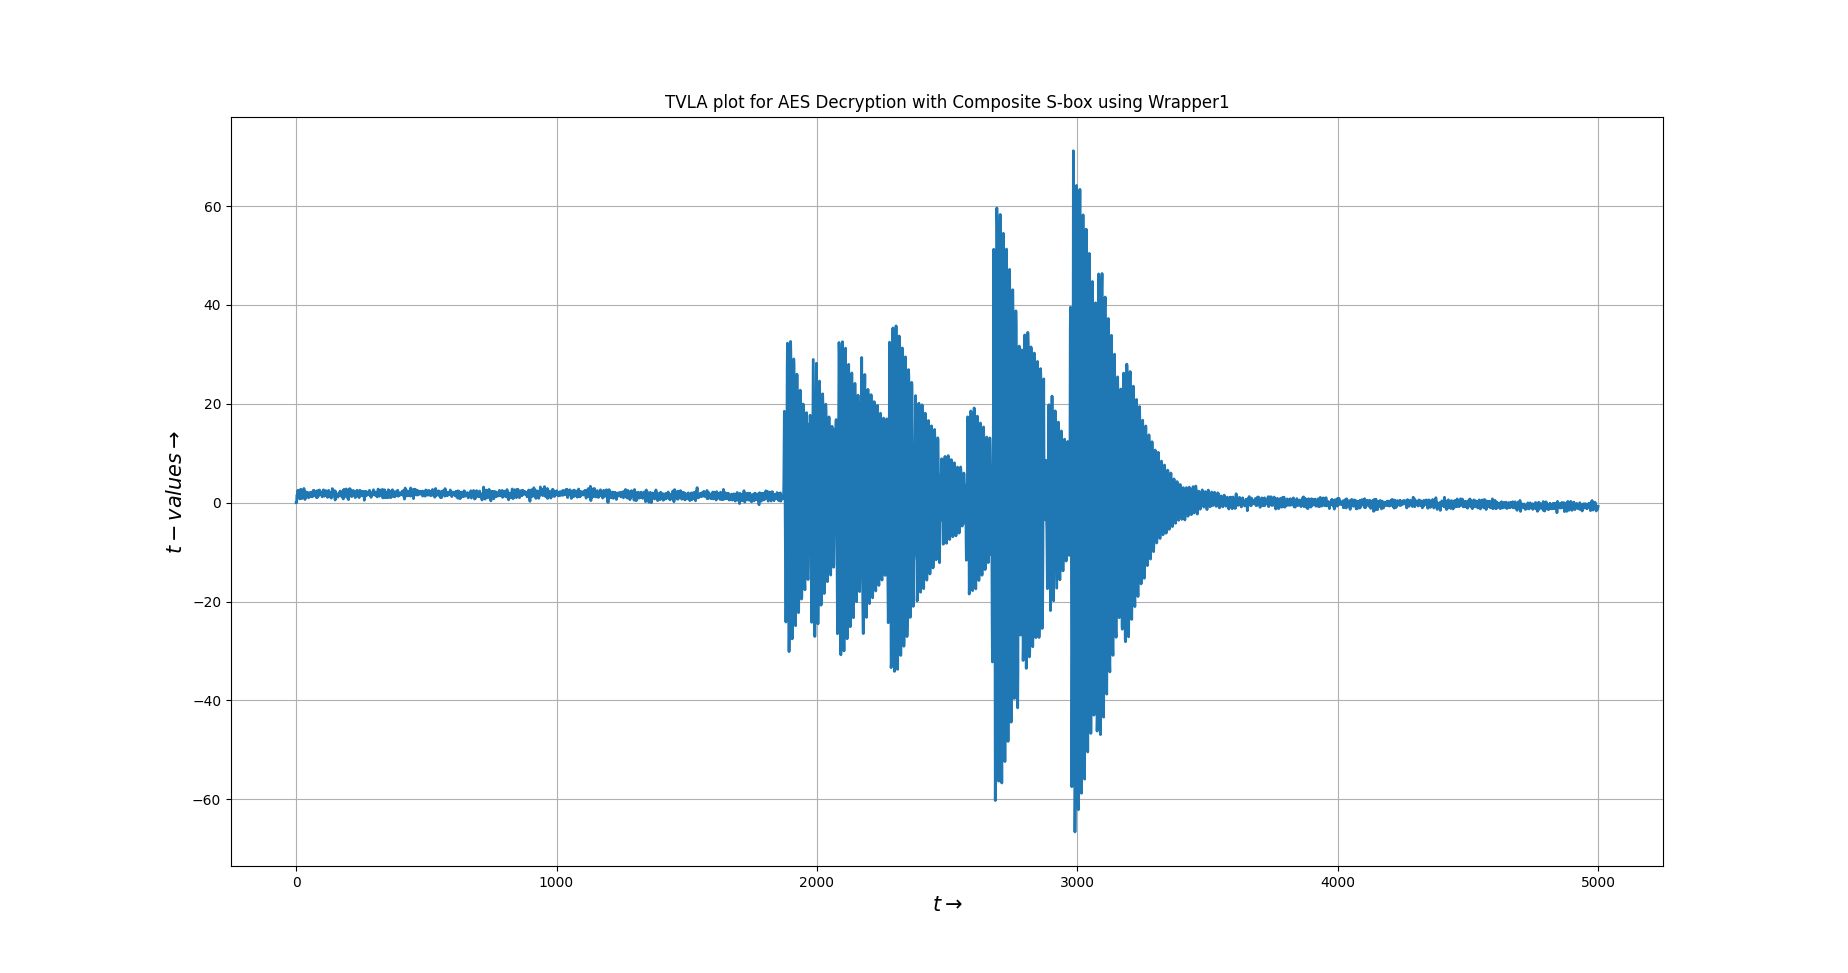
\includegraphics[scale=0.35]{report_pictures/temp_pics/Figure_11b}
\par\end{centering}
\caption{Plots for Encryption and Decryption process for Composite AES with
Wrapper1}
\end{figure}

TVLA scores were also calculated for Wrapper1.

\begin{table}[H]
\caption{TVLA scores for encryption with Composite AES using Wrapper1}

\centering{}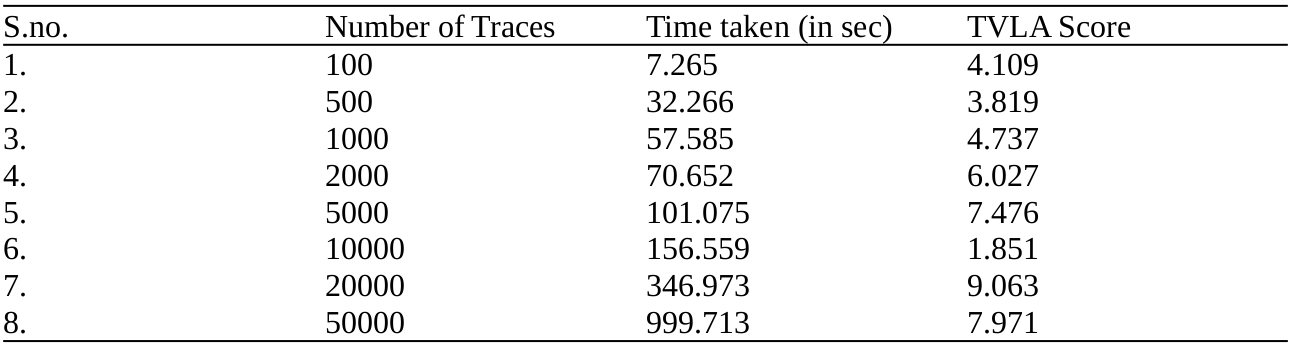
\includegraphics[scale=0.4]{report_pictures/sbox2_encr_w1}
\end{table}

\begin{table}[H]
\caption{TVLA scores for decryption with Composite AES using Wrapper1}

\centering{}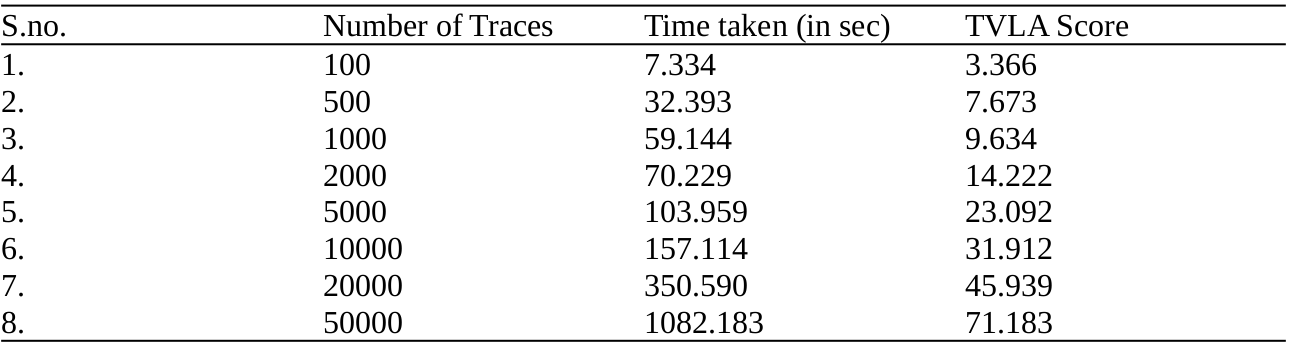
\includegraphics[scale=0.4]{report_pictures/sbox2_decr_w1}
\end{table}

\pagebreak{}

\subsubsection*{Evaluation with Wrapper2}

Following plots are the TVLA plots for encryption and decryption process
using Wrapper2. The sampling rate was at 10001 samples per trigger
for both the processes.
\begin{center}
\begin{figure}[H]
\centering{}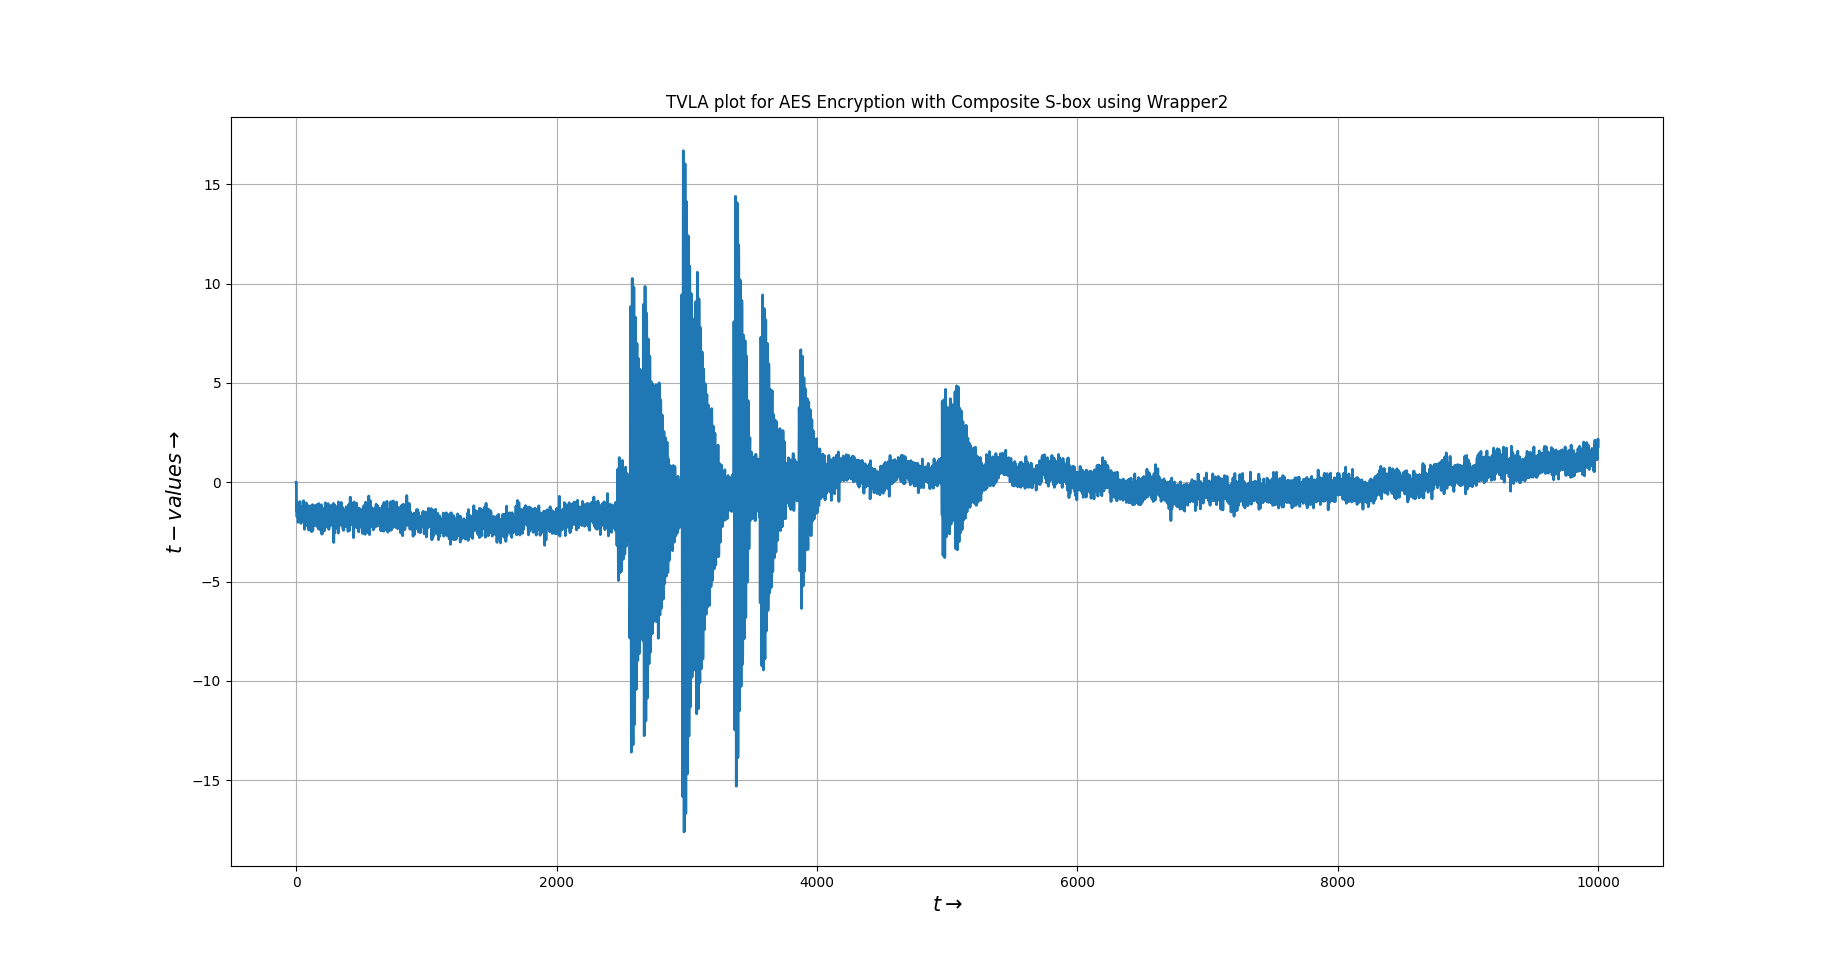
\includegraphics[scale=0.35]{report_pictures/temp_pics/Figure_10b}
\end{figure}
\par\end{center}

\begin{figure}[H]
\begin{centering}
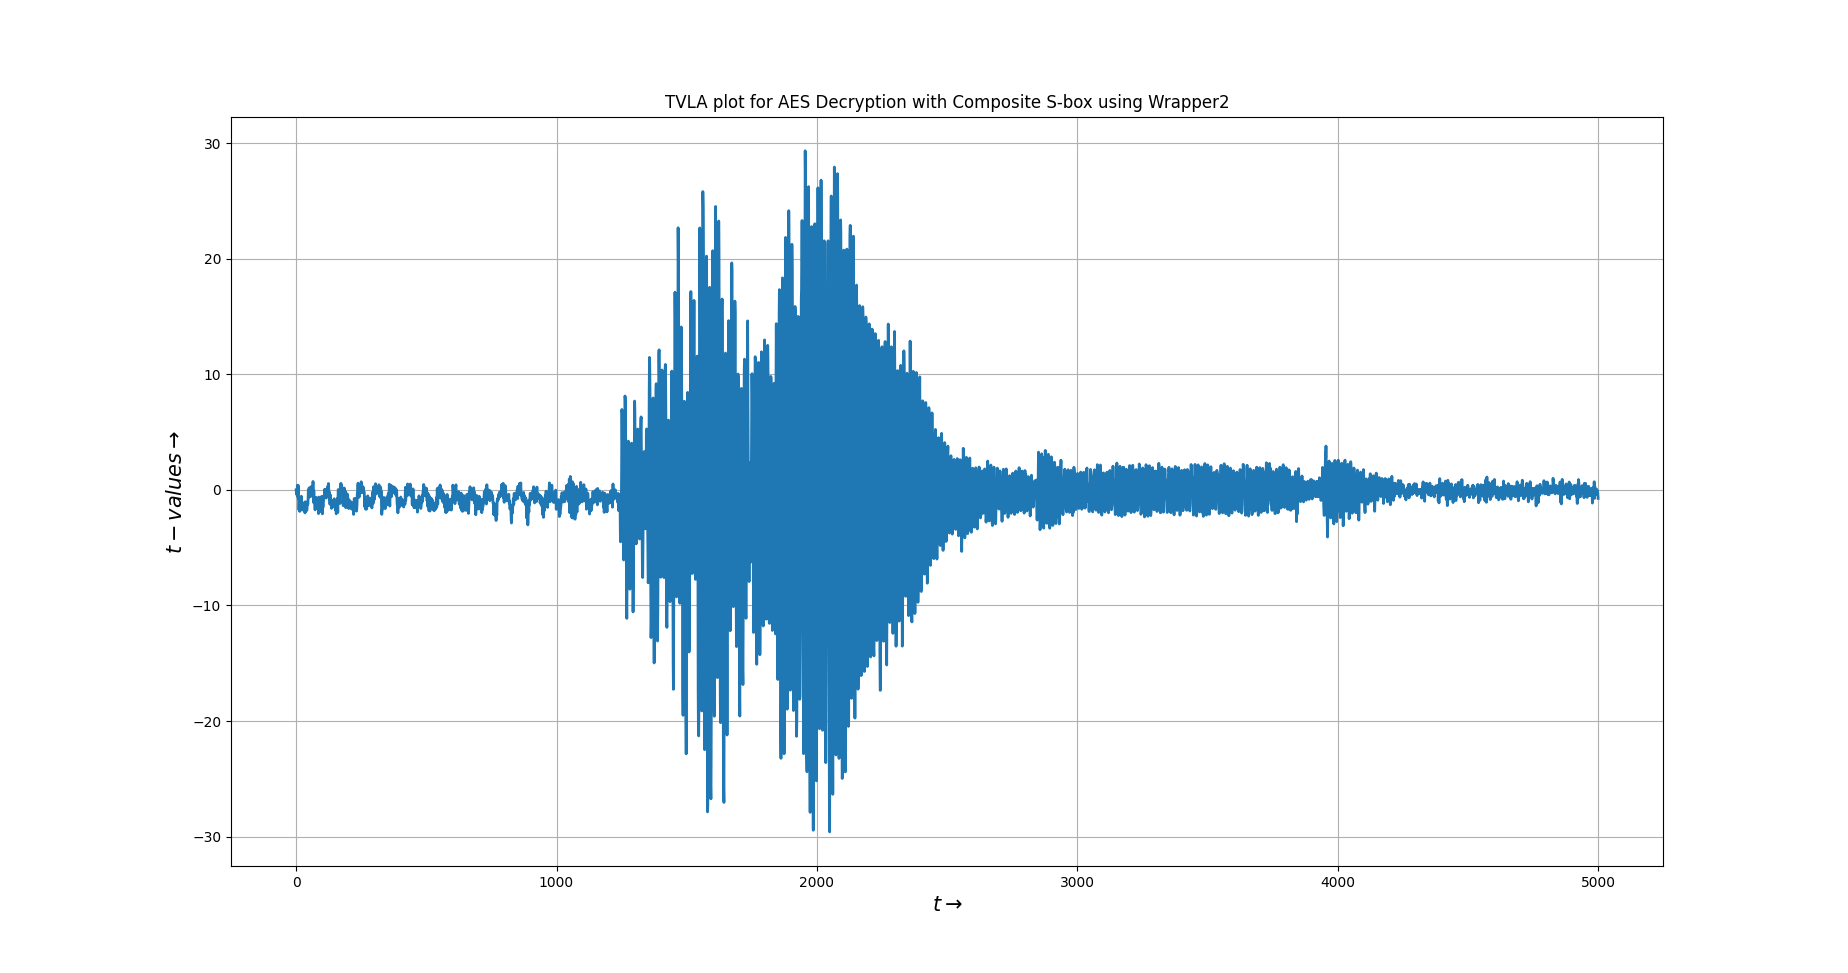
\includegraphics[scale=0.35]{report_pictures/temp_pics/Sbox2-Decr_modbnew}
\par\end{centering}
\caption{Plots for Encryption and Decryption process for Composite AES with
Wrapper2}

\end{figure}

\pagebreak{}

TVLA scores were also calculated for Wrapper2.

\begin{table}[H]
\caption{TVLA scores for encryption with Composite AES using Wrapper2}

\centering{}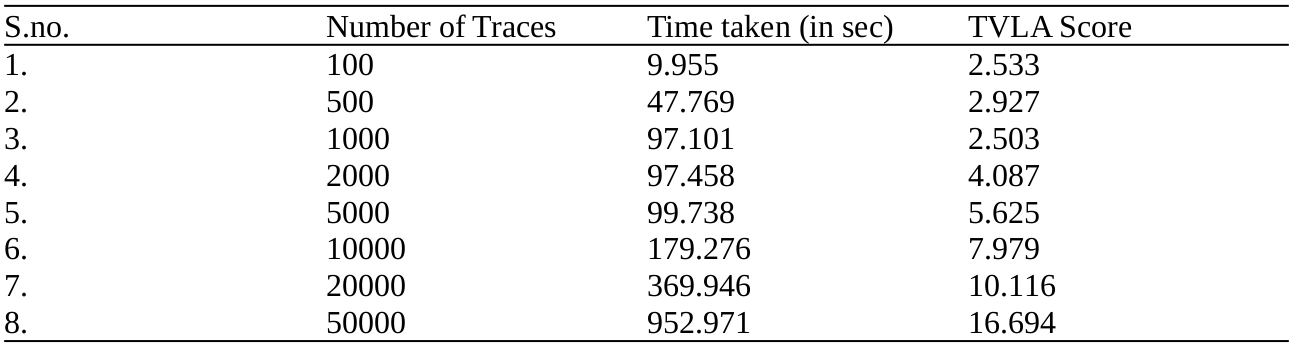
\includegraphics[scale=0.4]{report_pictures/sbox2_encr_w2}
\end{table}

\begin{table}[H]
\caption{TVLA scores for decryption with Composite AES using Wrapper2}

\centering{}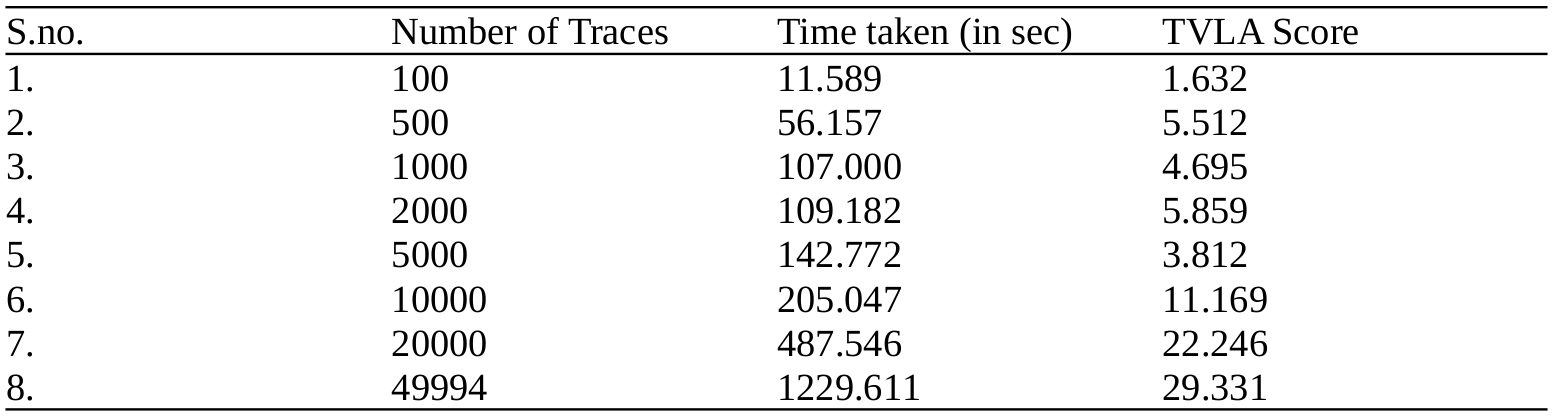
\includegraphics[scale=0.33]{report_pictures/sbox2_decr_mod}
\end{table}


\subsection{Evaluation of Threshold Implementation}

For the Threshold AES accelerator, approximately 5,00,000 traces were
collected for each dataset. The oscilloscope has a limit of collecting
a maximum of 1 lakh traces in each run and so we collected the output
in 10 batches by feeding 50,000 inputs from each dataset. The starting
random input for each batch was predetermined by simulating the Bluespec
code. Unlike the typical AES accelerator, the Threshold implementation
takes atleast 181 cycles for one AES process. We set the oscilloscope
to resolution of $5mV/div$ and $5\mu s/div$ and set the maximum
sampling rate at 10K samples per trigger. It was difficult to differentiate
between the cipher process's power signal and noise but at this resolution
some small peaks can be observed within the trigger range. From previous
TVLA analysis, we can notice the major impact on TVLA score because
of storing the AES output into registers within the trigger. Hence,
for this accelerator only Wrapper2 module was used and it has given
expected improvements. The implementation aspects can be found in
Section 3.4. For the python script, the number of cores is set to
$10$ and the width is set to $10000$.

Following plots are the TVLA plots for encryption and decryption process
using Wrapper2.
\begin{center}
\begin{figure}[H]
\centering{}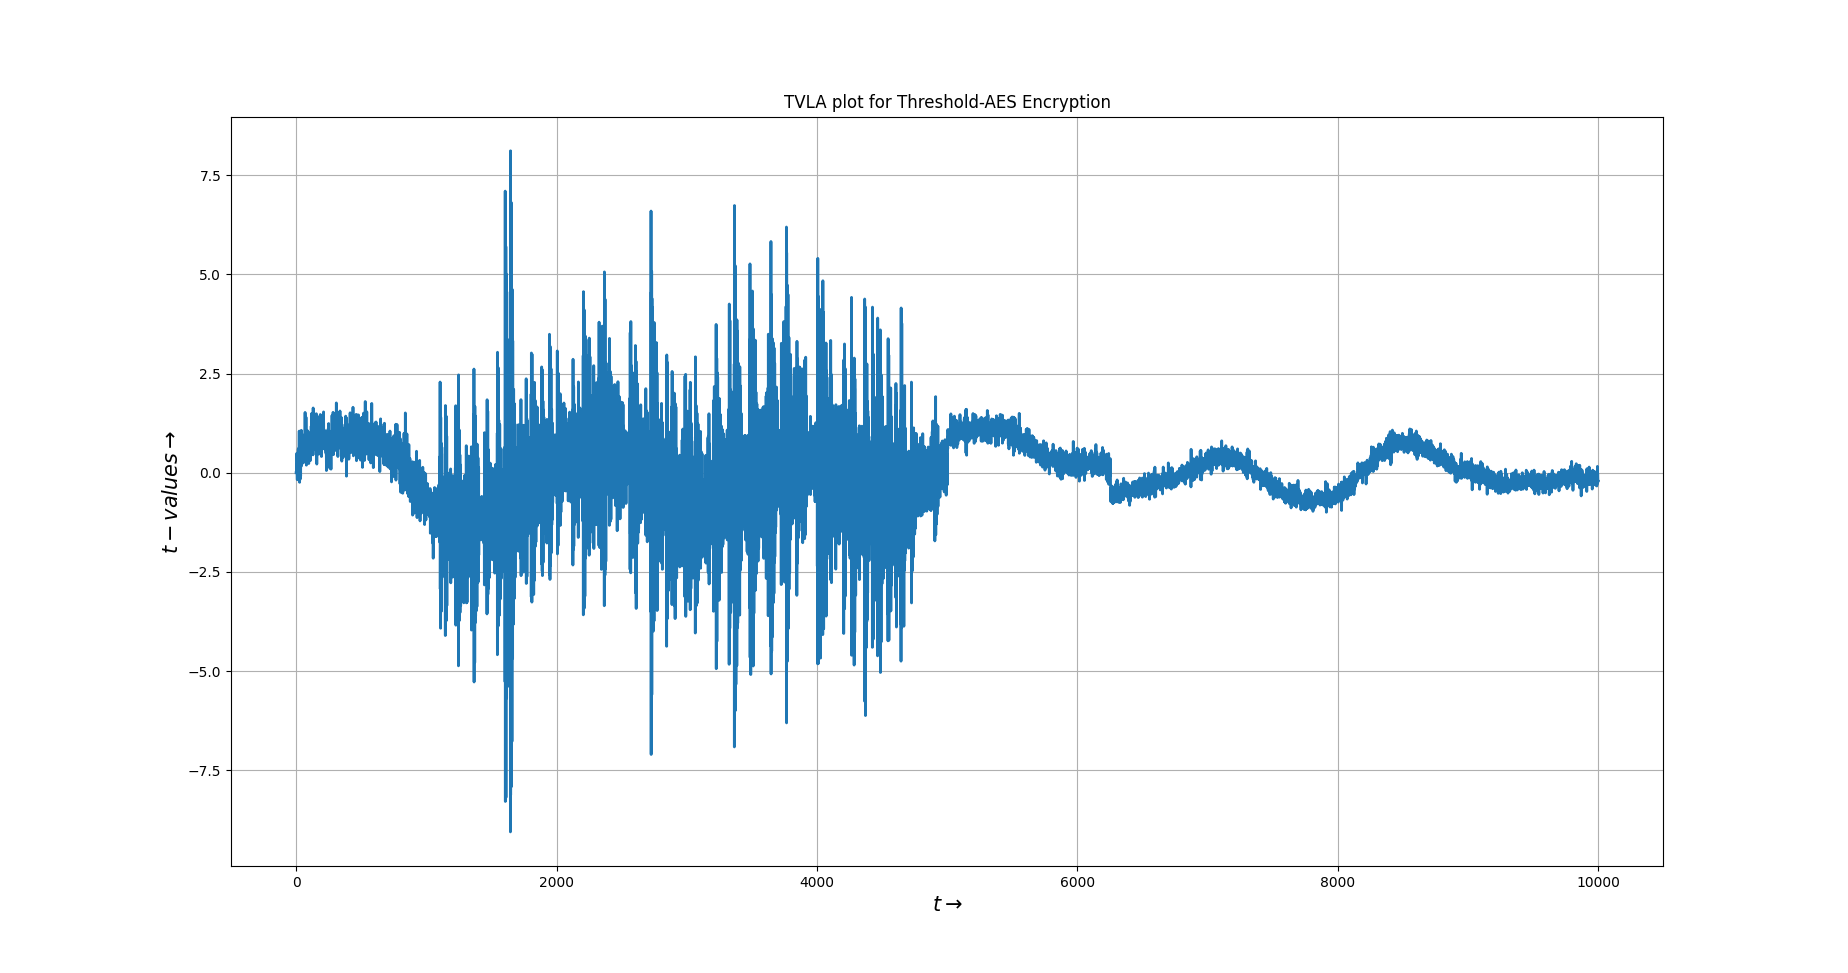
\includegraphics[scale=0.35]{report_pictures/temp_pics/Thresh-Encrb}
\end{figure}
\par\end{center}

\begin{figure}[H]
\begin{centering}
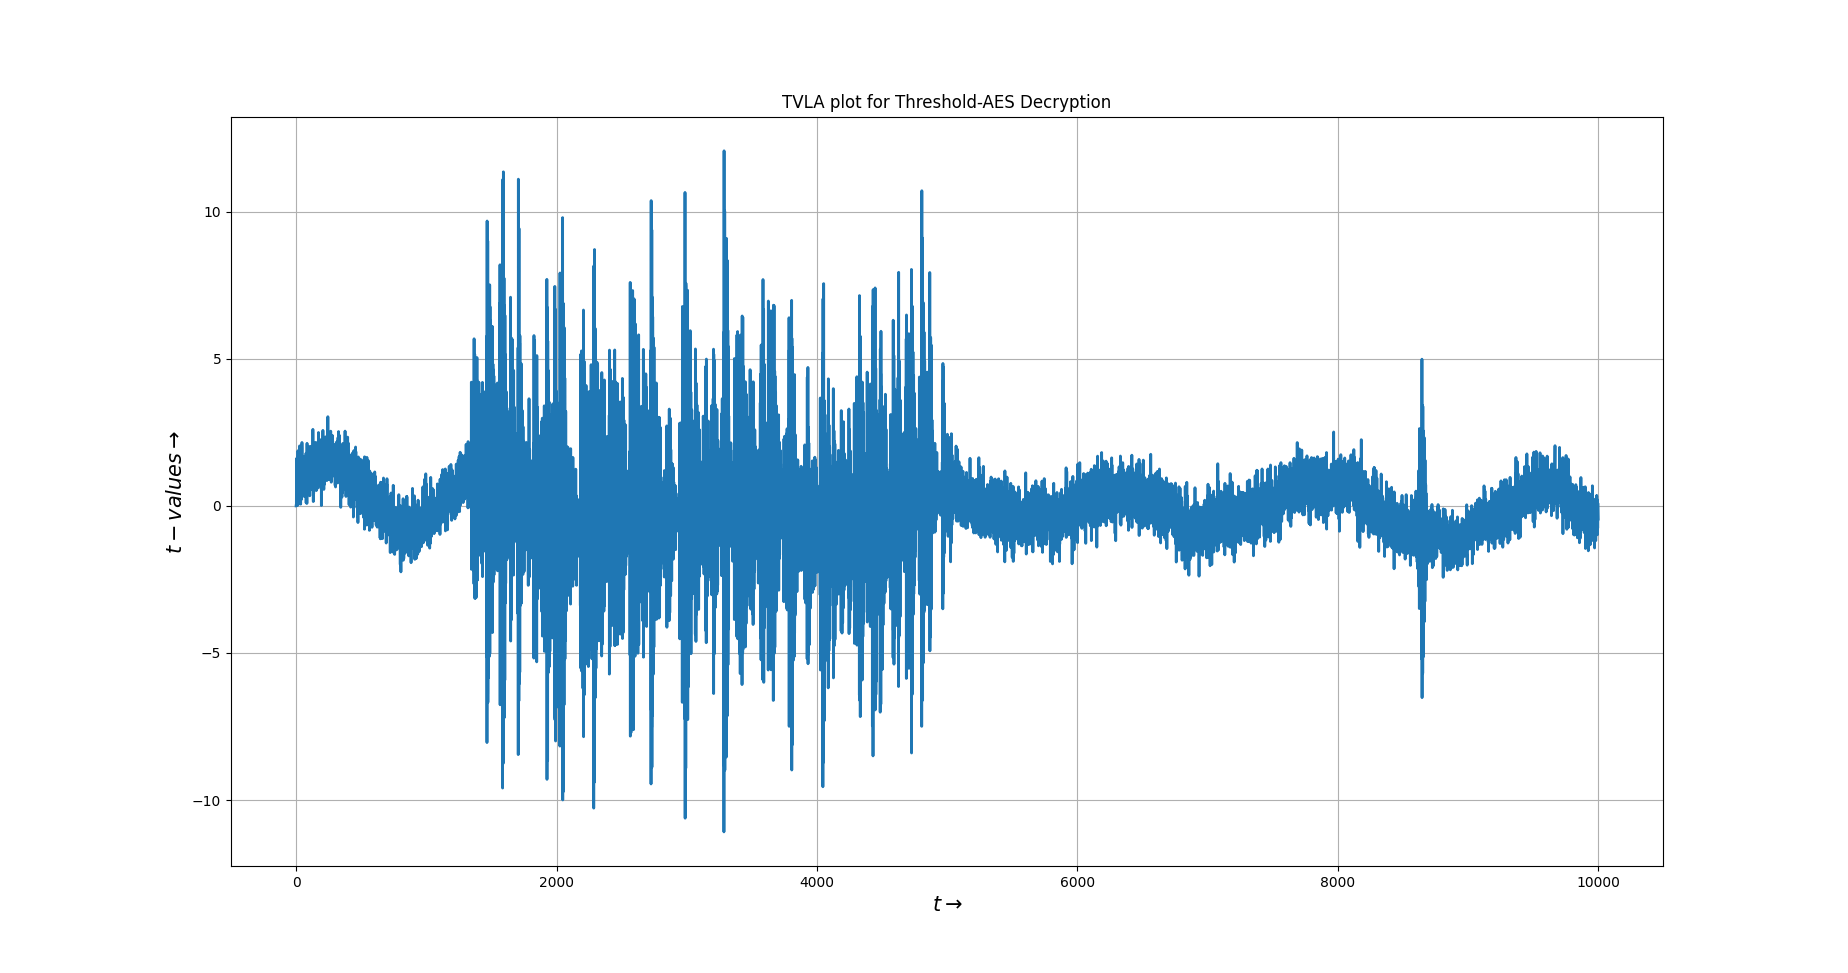
\includegraphics[scale=0.35]{report_pictures/temp_pics/Thresh-Decrb}
\par\end{centering}
\caption{Plots for Encryption and Decryption process for Threshold AES with
Wrapper2}

\end{figure}

TVLA scores were also calculated for Threshold AES accelerator with
Wrapper2.

\begin{table}[H]
\caption{TVLA scores for encryption with Threshold AES with Wrapper2}

\centering{}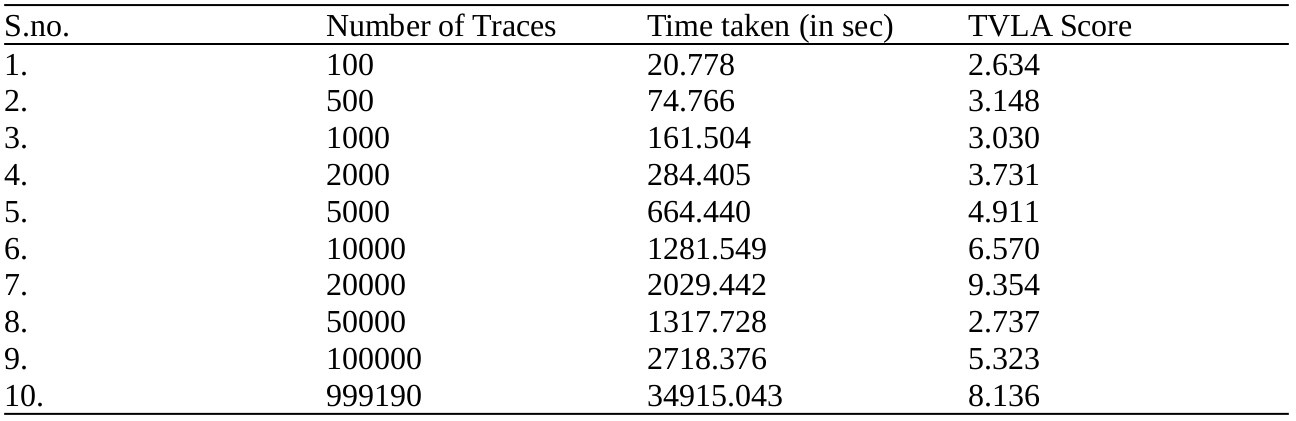
\includegraphics[scale=0.4]{report_pictures/thresh_encr}
\end{table}

\begin{table}[H]
\caption{TVLA scores for decryption with Threshold AES with Wrapper2}

\centering{}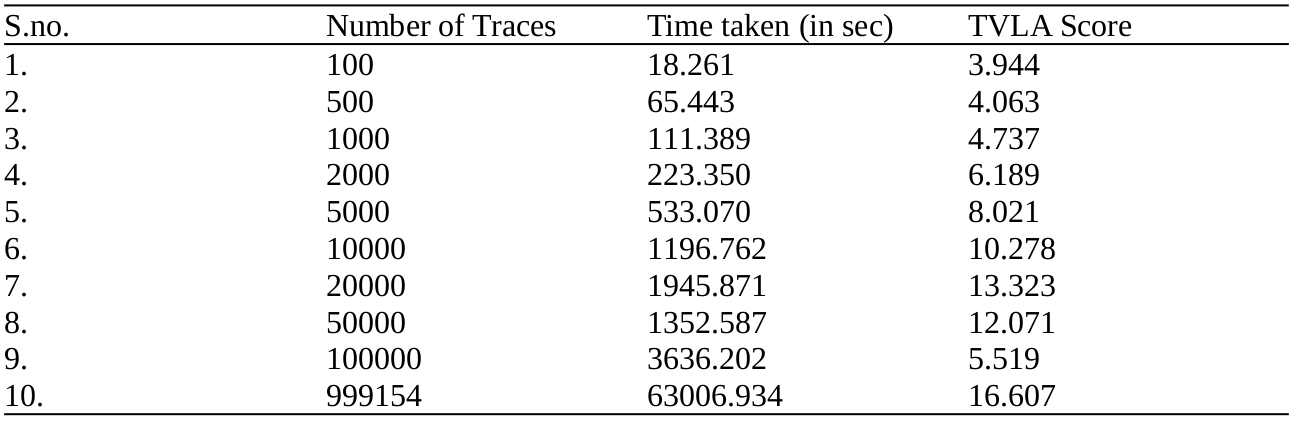
\includegraphics[scale=0.4]{report_pictures/thresh_decr}
\end{table}

Additionally, we have run the TVLA scripts for different width (same
number of cores) to see which is the most efficient. For this we have
used only the traces collected during encryption. We can see from
Table 14 that Width of around 1000 works most efficiently.

\begin{table}[H]
\caption{Analysis of width vs time taken for $\approx$1 lakh traces}

\centering{}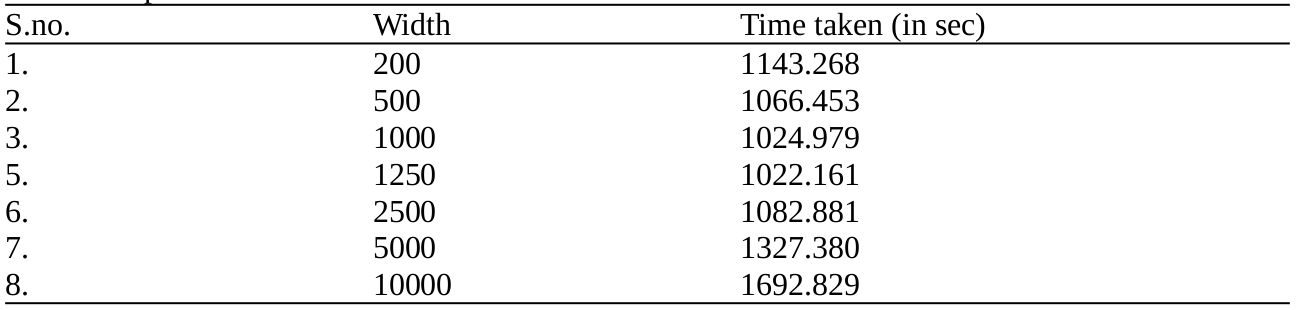
\includegraphics[scale=0.4]{report_pictures/time_1lakh}
\end{table}

\pagebreak{}

\section{Results and Conclusion}

Thus, we have evaluated three implementations of the AES accelerator
using the Welch's t-test which is the Lookup-table Based Implementation,
Composite Field Implementation and Threshold AES Implementation. From
our previous research \cite{key-1}, Composite Field implementation
is expected to be more secure than LUT based AES implementation. We
got the result as expected when we used Wrapper2 but the results were
ambiguous with Wrapper1.

\begin{table}[H]
\caption{Results between LUT based and Composite Field implementations for
50K traces}

\centering{}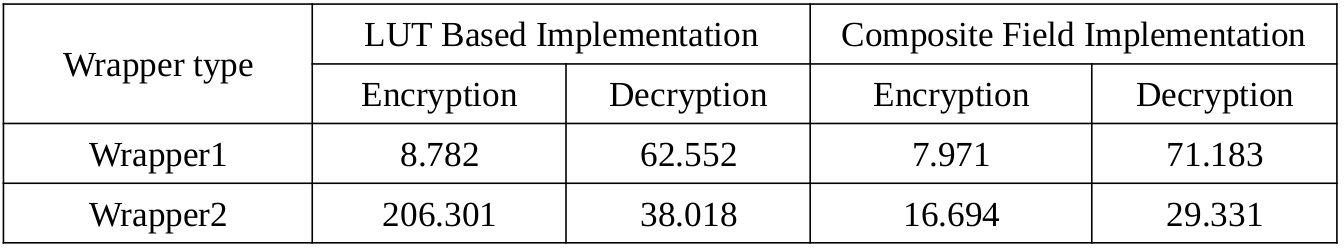
\includegraphics[scale=0.3]{report_pictures/conclusion1}
\end{table}

In Wrapper1 module, the following registers are changing during the
trigger:
\begin{itemize}
\item 2-bit \emph{mod\_state} changes during output stage and delay stage
\item 32-bit \emph{counter} increments once
\item 1-bit \emph{switcher}, to switch between fixed and random inputs,
gets toggled
\item 32-bit \emph{delayer} (delay counter) is set to 0
\item 128-bit \emph{input\_text} is updated with the cipher output if the
input was from the fixed dataset
\item 1-bit \emph{trigger} bit is also set to low
\end{itemize}
In Wrapper2 module, the following registers change during the trigger:
\begin{itemize}
\item 1-bit \emph{block} toggles once and is used to schedule the rules
in the Cipher Process 1 in Figure 9
\item 1-bit \emph{trigger} bit is set to low
\end{itemize}
Practically, we can expect as many registers as in Wrapper1 to get
updated in each cipher process but for TVLA we need to reduce the
role played by these dynamic changes in the net power consumption
to accurately evaluate the accelerator. Dynamic power consumption
due to register changes is significantly higher than power consumption
due to transistors \cite{key-7}. Though practically we don't see
much change in the power plots between the two wrappers, the effect
on TVLA is very significant. Hence, only Wrapper2 was used for Threshold
implementation and the result we have got is that it performs better
than Composite Field implementation. So overall, Threshold implementation
is the most secure among all three, followed by Composite Field implementation.

\begin{table}[H]
\caption{Comparison of all three implementations using Wrapper2 and with 50K
traces}

\centering{}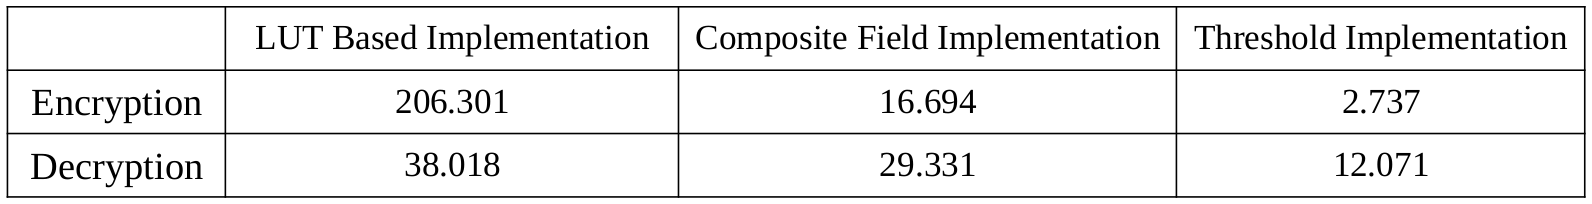
\includegraphics[scale=0.3]{report_pictures/conclusion2}
\end{table}

\pagebreak{}

We also conclude that the TVLA score increases with the number of
traces with the following Log-log plots in Figure 17. Threshold AES
will likely show more linearity at higher number of traces but we
can observe the general increase of maximum t-value with the number
of traces. With the values from the tables we can approximately show
that $t-value\propto\sqrt{N}$. 

\begin{figure}[H]
\begin{centering}
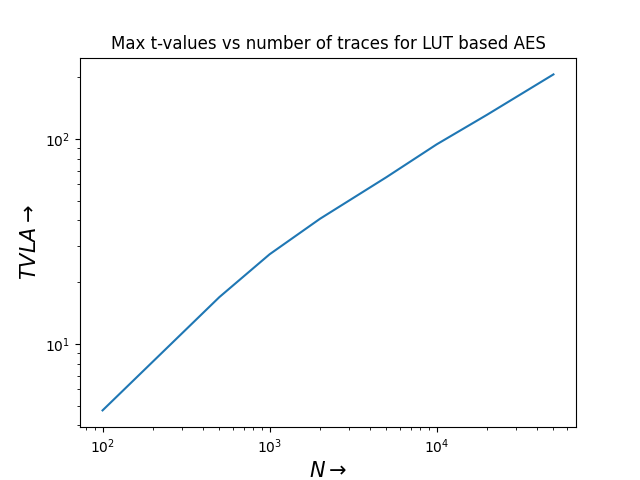
\includegraphics[scale=0.33]{report_pictures/tvla_LUT}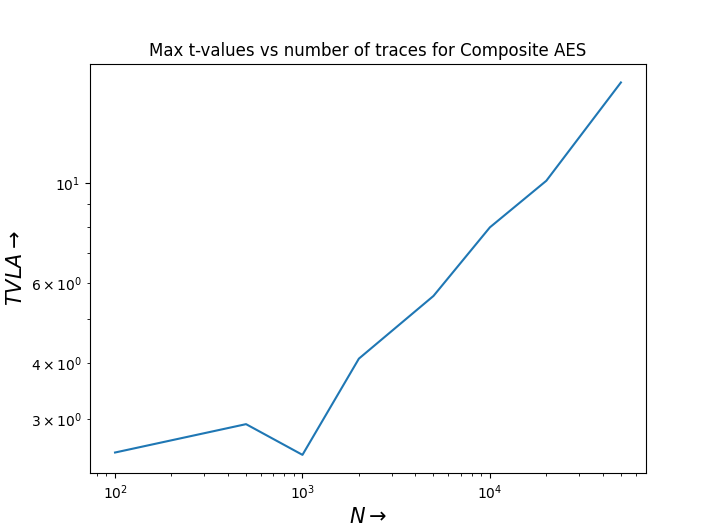
\includegraphics[scale=0.3]{report_pictures/tvla_Composite}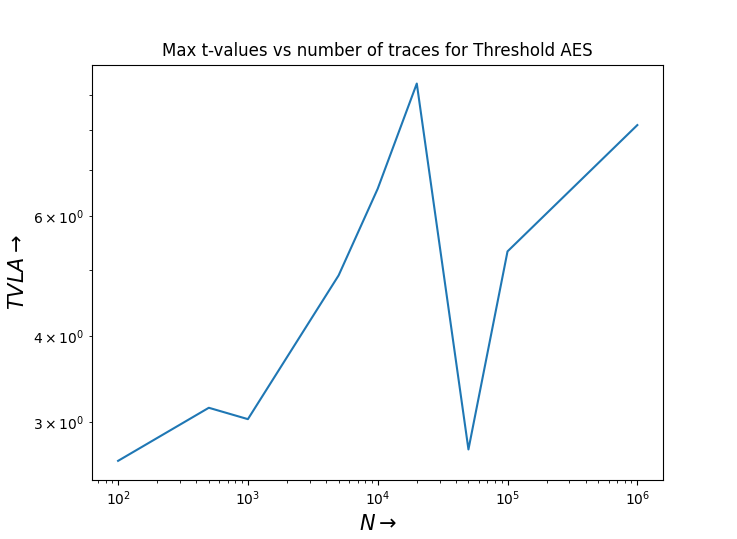
\includegraphics[scale=0.3]{report_pictures/tvla_thresh}
\par\end{centering}
\caption{Log-log plots for the three implementations}

\end{figure}


\section{Scope of improvement}
\begin{enumerate}
\item \textbf{Remote setup for the oscilloscope for viewing the StartDSO
application:} Instruments operation and trace data collection can
be done through remote operation using TCP-IP, ActiveDSO, GP-IB, etc.
\item \textbf{Effect of routing algorithms used:} We have used only default
synthesis and implementation for our analysis. The effect could be
significant if, say, Speed Maximized synthesis option is used which
has higher power consumption \cite{key-5}.
\item \textbf{Analysis of the dependence of TVLA on the frequency of the
FPGA board:} Very low frequency was used because of various limitations
as stated previously. Higher frequency implies higher power consumption
and this could have its own implications.
\item \textbf{Practical assessment of accelerators by collecting traces
when it is integrated with a CPU:} The Typical AES accelerator has
been integrated with Shakti C-Class and system functions have been
provided to allow setting of the trigger pin. The problem with using
a CPU is that it will take more time to synthesise and implement as
compared to the wrapper modules and modifications to the CPU might
be necessary to limit the total number of LUT usage to less than 110,000
LUTs (total number of LUTs in the SASEBO-GIII platform).
\item \textbf{To improve threshold implementation:} Specific operations
which are causing the leakage can be identified by detailed analysis
of the TVLA plots and can be used to improve threshold implementation.
\end{enumerate}
\pagebreak{}

\section{Appendix}

Limitations of this study are as follows:
\begin{itemize}
\item TVLA value was not very steady and it is possible that the TVLA score
could change significantly when a test is run multiple times: A large
number of tests might be required to get a consistent value. The physical
conditions of the setup could also play a role in the trace collection.
\item Frequency of the FPGA board had to be set to minimum due to the limit
on the maximum sampling rate: Large number of samples had to be collected
for a small process which takes only 12 cycles. This causes some traces
to be skipped in the beginning/end, and the process was repeated if
sufficient number of traces were not recorded.
\item The limited RAM capacity of the oscilloscope caused intermittent hanging
of the set up, causing repetition of the validity of collected data
and loss of time.
\end{itemize}
\begin{thebibliography}{1}
\bibitem{key-1} Aditya Pradeep, Vishal Mohanty, Adarsh Muthuveeru
Subramaniam, and Chester Rebeiro (2019), \textquoteleft Revisiting
AES S-Box Composite Field Implementations for FPGAs\textquoteright ,
IEEE Embedded System Letters, Vol.11, No.3.

\bibitem{key-5} Akhil Sai and Chester Rebeiro (2017), \textquoteleft Influence
of CAD Routing Algorithms on Cryptographic Side Channel Attacks\textquoteright ,
Department of Computer Science and Engineering, IIT Madras.

\bibitem{key-6} Gilbert Goodwill, Benjamin Jun, Josh Jaffe and Pankaj
Rohatgi, \textquoteleft A testing methodology for side-channel resistance
validation\textquoteright , Cryptography Research Inc.

\bibitem{key-7} Stefan Mangard, Elisabeth Oswald and Thomas Popp,
\textquoteleft Power Analysis Attacks: Revealing the Secrets of Smart
Cards\textquoteright , Textbook.

\bibitem{key-11} Vishal Mohanty and Chester Reberio (2019), \textquoteleft Efficient
AES Threshold Implementation on FPGA\textquoteright , UGRC-II report,
Department of Computer Science and Engineering, IIT Madras.
\end{thebibliography}

\end{document}
